\documentclass[12pt]{article}

\author{Matthew D. Cocci}
\title{Asset Pricing}
\date{\today}

%% Formatting & Spacing %%%%%%%%%%%%%%%%%%%%%%%%%%%%%%%%%%%%

%\usepackage[top=1in, bottom=1in, left=1in, right=1in]{geometry} % most detailed page formatting control
\usepackage{fullpage} % Simpler than using the geometry package; std effect
\usepackage{setspace}
%\onehalfspacing
\usepackage{microtype}

%% Formatting %%%%%%%%%%%%%%%%%%%%%%%%%%%%%%%%%%%%%%%%%%%%%

%\usepackage[margin=1in]{geometry}
    %   Adjust the margins with geometry package
%\usepackage{pdflscape}
    %   Allows landscape pages
%\usepackage{layout}
    %   Allows plotting of picture of formatting



%% Header %%%%%%%%%%%%%%%%%%%%%%%%%%%%%%%%%%%%%%%%%%%%%%%%%

%\usepackage{fancyhdr}
%\pagestyle{fancy}
%\lhead{}
%\rhead{}
%\chead{}
%\setlength{\headheight}{15.2pt}
    %   Make the header bigger to avoid overlap

%\fancyhf{}
    %   Erase header settings

%\renewcommand{\headrulewidth}{0.3pt}
    %   Width of the line

%\setlength{\headsep}{0.2in}
    %   Distance from line to text


%% Mathematics Related %%%%%%%%%%%%%%%%%%%%%%%%%%%%%%%%%%%

\usepackage{amsmath}
\usepackage{amsfonts}
\usepackage{mathrsfs}
\usepackage{amsthm} %allows for labeling of theorems
\theoremstyle{plain}
\newtheorem{thm}{Theorem}[section]
\newtheorem{lem}[thm]{Lemma}
\newtheorem{prop}[thm]{Proposition}
\newtheorem{cor}[thm]{Corollary}
\newtheorem{ax}[thm]{Axiom}

\theoremstyle{definition}
\newtheorem{defn}[thm]{Definition}
\newtheorem{ex}[thm]{Example}

\theoremstyle{remark}
\newtheorem*{rmk}{Remark}
\newtheorem*{note}{Note}

% Below supports left-right alignment in matrices so the negative
% signs don't look bad
\makeatletter
\renewcommand*\env@matrix[1][c]{\hskip -\arraycolsep
  \let\@ifnextchar\new@ifnextchar
  \array{*\c@MaxMatrixCols #1}}
\makeatother


%% Font Choices %%%%%%%%%%%%%%%%%%%%%%%%%%%%%%%%%%%%%%%%%

\usepackage[T1]{fontenc}
\usepackage{lmodern}
\usepackage[utf8]{inputenc}
%\usepackage{blindtext}


%% Figures %%%%%%%%%%%%%%%%%%%%%%%%%%%%%%%%%%%%%%%%%%%%%%

\usepackage{graphicx}
\usepackage{subfigure}
    %   For plotting multiple figures at once
%\graphicspath{ {Directory/} }
    %   Set a directory for where to look for figures


%% Hyperlinks %%%%%%%%%%%%%%%%%%%%%%%%%%%%%%%%%%%%%%%%%%%%
\usepackage{hyperref}
\hypersetup{%
    colorlinks,
        %   This colors the links themselves, not boxes
    citecolor=black,
        %   Everything here and below changes link colors
    filecolor=black,
    linkcolor=black,
    urlcolor=black
}

%% Colors %%%%%%%%%%%%%%%%%%%%%%%%%%%%%%%%%%%%%%%%%%%%%%%

\usepackage{color}
\definecolor{codegreen}{RGB}{28,172,0}
\definecolor{codelilas}{RGB}{170,55,241}


%% Including Code %%%%%%%%%%%%%%%%%%%%%%%%%%%%%%%%%%%%%%%

\usepackage{verbatim}
    %   For including verbatim code from files, no colors
\usepackage{listings}
    %   For including code snippets written directly in this doc

\lstdefinestyle{bash}{%
  language=bash,%
  basicstyle=\ttfamily,%
  showstringspaces=false,%
  commentstyle=\color{gray},%
  keywordstyle=\color{blue},%
  xleftmargin=0.25in,%
  xrightmargin=0.25in
}

\definecolor{codegreen}{RGB}{28,172,0}
\definecolor{codelilas}{RGB}{170,55,241}
\newcommand{\matlabcode}[1]{%
    \lstset{language=Matlab,%
        basicstyle=\footnotesize,%
        breaklines=true,%
        morekeywords={matlab2tikz},%
        keywordstyle=\color{blue},%
        morekeywords=[2]{1}, keywordstyle=[2]{\color{black}},%
        identifierstyle=\color{black},%
        stringstyle=\color{codelilas},%
        commentstyle=\color{codegreen},%
        showstringspaces=false,%
            %   Without this there will be a symbol in
            %   the places where there is a space
        numbers=left,%
        numberstyle={\tiny \color{black}},%
            %   Size of the numbers
        numbersep=9pt,%
            %   Defines how far the numbers are from the text
        emph=[1]{for,end,break,switch,case},emphstyle=[1]\color{red},%
            %   Some words to emphasise
    }%
    \lstinputlisting{#1}
}
    %   For including Matlab code from .m file with colors,
    %   line numbering, etc.

%% Bibliographies %%%%%%%%%%%%%%%%%%%%%%%%%%%%%%%%%%%%

%\usepackage{natbib}
    %---For bibliographies
%\setlength{\bibsep}{3pt} % Set how far apart bibentries are

%% Misc %%%%%%%%%%%%%%%%%%%%%%%%%%%%%%%%%%%%%%%%%%%%%%

\usepackage{enumitem}
    %   Has to do with enumeration
\usepackage{appendix}
%\usepackage{natbib}
    %   For bibliographies
\usepackage{pdfpages}
    %   For including whole pdf pages as a page in doc


%% User Defined %%%%%%%%%%%%%%%%%%%%%%%%%%%%%%%%%%%%%%%%%%

%\newcommand{\nameofcmd}{Text to display}
\newcommand*{\Chi}{\mbox{\large$\chi$}} %big chi
    %   Bigger Chi



%%%%%%%%%%%%%%%%%%%%%%%%%%%%%%%%%%%%%%%%%%%%%%%%%%%%%%%%%%%%%%%%%%%%%%%%
%% BODY %%%%%%%%%%%%%%%%%%%%%%%%%%%%%%%%%%%%%%%%%%%%%%%%%%%%%%%%%%%%%%%%
%%%%%%%%%%%%%%%%%%%%%%%%%%%%%%%%%%%%%%%%%%%%%%%%%%%%%%%%%%%%%%%%%%%%%%%%



\begin{document}
\maketitle

\tableofcontents

\newpage
\section{Stochastic Calculus Review}

\newpage
\section{Introduction}

If all of Asset Pricing needed to be reduced to one simple,
general, yet wholly appropriate epithet, a decent starting
point would be ``Price equals expected discounted payoff.''
\\
\\
To segment the discussion further, John Cochrane (whose Asset pricing book
these notes are based on) suggests the following two classes of pricing
approaches:
\begin{enumerate}
    \item {\sl Absolute Pricing}: ``Pricing assets by exposure
	to fundamental sources of macroeconomic risk.'' This
	approach includes general equilibrium models.
    \item {\sl Relative Pricing}: This type of pricing considers
	only how an asset should be priced relative to
	other assets that can be bought and sold in the
	market. Black-Scholes and any arbitrage arguments
	would fall under this category.
\end{enumerate}
However, many asset pricing approaches are a blend of the two.
\\
\\
To be more specific, we can reduce asset pricing to two
equations:
\begin{equation}
    P_t = E[M_{t+1} X_{t+1} ]
\end{equation}
\begin{equation}
    M_{t+1} = f(\text{data, parameters})
\end{equation}
where $P_t$ is the asset price, $X_{t+1}$ is the asset's payoff,
and $M_{t+1}$ is the stochastic discount factor.
This approach joins together what used to be separate theories so
that pricing stocks, bonds, and options now represent special
cases of this more general framework summarized by the equations above.


\section{Asset Pricing Facts}

There are a number of empirical observations that have been made
over the years, and this section will detail their conclusions
and main insights.

\subsection{Equity Premium and Risk}

We'll beging by thinking about the \emph{Equity Premium}, which
is the returns to stocks above and beyond bonds (so if you borrow
in bonds and lend in stocks): $E[R^{\text{stocks}}-R^{\text{bonds}}]$.
Here are the facts:
\begin{enumerate}
    \item The equity premium is \emph{big}, about 7\%.
    \item There's a lot of risk in stocks: there's a greater
	standard deviation in returns (although we'll think about
	risk a bit differently). Stock returns are also correlated
	with macro variables.
    \item Compared with stocks returns, GDP and Consumption growth are much
	more stable, though they do vary a bit (with the standard deviation
	being much closer to bond returns' volatility than stock returns).
\end{enumerate}

\subsection{Time-Varying Risk Premium}

Now we want to consider what explains the Equity Premium. For that,
we regress returns on some signal we hope will explain future returns.
Here's a few regressions. The main result will be that
\emph{excess returns} are forecastable---that is, the time-varying
reward for risk can be forecast. We're not forecasting raw rate.
Now onto facts:
\begin{enumerate}
    \item {\sl Old View}: Regression of returns on lagged returns:
	    \[ R_{t+1} = a + b R_t + \varepsilon_{t+1} \]
	This regresion typically yields a value for $b$ around
	0, in which case future returns given returns today
	are more or less \emph{random}.  The main result:
	\begin{equation}
	    \label{oldview}
	    ER_{t+1} = E[a + 0\cdot R_t + \varepsilon_{t+1}] = a
	\end{equation}
	in which case \emph{expected returns} are large and constant.
    \item {\sl New View}: The old view, encapsulated in Equation \ref{oldview},
	drove theory for many years. But now, we have a different
	picture: there are variables that forecast stock returns.
	Now, we run the regression
	\begin{equation}
	    \label{newview}
	    R^e_{t\rightarrow t+k} = a + b \left(\frac{D_t}{P_t}\right)
		+ \varepsilon_{t+k}
	\end{equation}
	where $R^e$ is the excess return over bonds, $D_t$ is current
	dividends, and $P_t$ is current price. From this regression,
	we get a large, positive regression coefficient.
	So we actually \emph{can} predict returns over the business
	cycle via this dividend/price ratio (but it's still tough
	in the short run).

    \item {\sl New View Interpretation}: The dividend yield $(D_t/P_t)$, which
	is the inverse of prices, turns out to vary a lot over time.
	Moreover, if you buy when the dividend yield ratio is
	\emph{high} (so that prices are low), you will earn high
	returns in expectation.  Vice versa for a low dividend yield
	ratio (so high prices).

	Moreover, we can get the standard deviation in the expected returns over
	time, which is the fitted value $ER^e_{t\rightarrow t+k} = a + b
	E\left(D_t/P_t\right)$ from Equation \ref{newview}. It turns
	out that expected returns \emph{also vary}, and they vary
	\emph{substatially}, at about 6\%.

	Recall that it was puzzling
	that stocks should earn 7\% over bonds. Now we're saying that
	they earn 7\% over bonds \emph{and} vary with a standard
	deviation of about 6\% a year. Average \emph{changes} in
	$ER^e_{t\rightarrow t+k}$ are about as much as the average
	confounding \emph{level}.\footnote{Of course, \emph{actual}
	returns vary even more than expected returns---recall about
	17\%.}
    \item {\sl Why do prices vary?}: We know that the dividend/price
	ratio varies a lot, but it's mostly driven by prices. Why?
	Well, we used to think
	\begin{equation}
	    \label{oldidea}
	    \text{High Prices} \Rightarrow \text{High Future Growth}
		\Rightarrow \text{High E[Future Dividends]}
	\end{equation}
	But if we run the regression implied by Equation \ref{oldidea},
	\begin{equation}
	    \label{oldideareg}
	    \frac{D_{t+k}}{D_t} = a + b \left(\frac{D_t}{P_t}\right)
		+ \varepsilon_{t+k}
	\end{equation}
	we find out that the logic of \ref{oldidea} is \textbf{wrong}.
	The regression coefficient in Equation \ref{oldideareg} is
	negligible and there is no explanatory power (as
	reflected in the $R^2$).  So actaully
	\begin{equation}
	    \label{newidea}
	    \text{High Prices} \Rightarrow \text{Low Future E[Returns]}
	\end{equation}
	So it's not that dividends will adjust if prices are high
	and low---dividends are remarkably stable relative to prices!
	Instead, \emph{prices} will adjust.
	\\
	\\
	In short: high prices are correlated with a good economy,
	when people are willing to bear more risk.  So returns will
	be low. Vice versa for low prices.
\end{enumerate}


\subsection{The Cross Section of Stock Returns}

We talked about returns over time in the previous sections. Now
let's consider the facts about how returns vary \emph{across assets}
at a given time.
\begin{enumerate}
    \item {\sl Market Cap}: Small stocks earn more on average than
	large stocks.  They are also riskier.
    \item {\sl Growth vs. Value}: Value stocks (high book to value)
	tend to earn more.
    \item {\sl Capital Asset Pricing Model}: This model predicts
	returns based on the correlation between the asset and
	the market portfolio.
    \item {\sl Multifactor Model}: This model was put forward by
	Fama and French to capture the extra variation in returns
	that the Capital Asset Pricing Model failed to explain.
	This is the modern view. Specifically, Fama and French posit
	\begin{equation}
	    \label{ff3fm}
	    ER^{e,i} = \alpha_i + b_iE[R^m - R^f] + h_i E(\text{hml})
		+ s_i E(\text{smb})
	\end{equation}
	where $E($hml$)$ represents ``high minus low'' (for
	value minus growth stocks)
	and $E($smb$)$ for ``small minus big'' (for market cap).
    \item {\sl Stock Market Volatility:} We used to think volatility
	was pretty constant over time.  Now we know that the
	variance of returns changes over time.
\end{enumerate}

\clearpage
\section{Asset Pricing Theory Overview: $p=E(mx)$}

This section is about understanding the fundamental formula for
all of asset pricing, where an \emph{asset} is anything
that promises a future stream of payments:
\begin{equation}
    \label{pemx}
    p_t = \mathbb{E}_t[m_{t+1} x_{t+1}]
\end{equation}
This is huge because it lets us define a \emph{single} stochastic
discount factor $m_{t+1}$ for everything. So the price of \emph{any
asset} is determined by the expectation of its payoffs, weighted and
adjusted for risk by $m_{t+1}$.

\subsection{Utility and the Investor's Objective Function}

So first, we'll consider a simple utility function for two-period
consumption, which covers $t$ and $t+1$---the relevant time periods
in Equation~\ref{pemx}. Spefically, we'll define
\begin{equation}
    \label{util}
    U(c_t, c_{t+1}) = u(c_t) + \beta \;\mathbb{E}_t\left[u(c_{t+1})\right]
\end{equation}
where $\beta$ is the discount factor with respect to \emph{time} (how
much an investor discounts a dollar tomorrow), \textbf{not} risk which
will depend upon the shape of the utility function. Note that
Equation~\ref{util} above is a very simple utility function which we can
generalize further if we so choose. See Section for a discussion of
non-separabilities in utility with an example where the investor values
high leisure as well, not just consumption in isolation.
\\
\\
For the \emph{internal}, one-period utility function, $u(\cdot)$, we'll
want the normal properties of utility, $u'>0$ and $u''<0$, which can be
expressed in the simple, often-useful \emph{power utility} function
\begin{equation}
    \label{upwr}
    u(c) = \frac{c^{1-\gamma}-1}{1-\gamma} \quad\Rightarrow\quad
	u'(c) = c^{-\gamma}
\end{equation}
This utility function also has the property that as
$\lim_{\gamma\rightarrow 1}u(c) = \ln c$.

\subsection{Understanding the Components}

Now let's take each component of Equation~\ref{pemx} in turn
before we derive it:
\begin{enumerate}
  \item $x_{t+1}$: This is the \emph{payoff} at time $t+1$ in gross
    terms (values like 1.10), not net, log, or percentage (like 0.1,
    $\log(1.1)$, or 10\%).  Often, $x_{t+1}$ will be a random variable
    that depends upon the state of nature at time $t+1$.

  \item $p_t$: To get the payoff, $x_t$, you have to pay some price
    $p_t$ today. Note that it is possible for $p_t$ to equal 0, like in
    a bet (nothing today, +1 tomorrow if I win, -1 if I lose).  No money
    changes hands.

  \item $m_{t+1}$: Recall Equation~\ref{util} above.  It left us free
    parameters, $\beta$ and $\gamma$, which allow us to tweak
    ``impatience,'' or time sensitivity of consumption ($\beta$), as
    well as risk-aversion via curvature in the utility function
    ($\gamma$).  This gives us everything we need to charactertize the
    stochastic discount factor, $m_{t+1}$, which is a generalization of
    non-risk-adjusted discount factors. Lots more on this later.
\end{enumerate}
Here's a table reproduced from Cochrane's book that shows how we can
accommodate pretty much any asset within the $p_t$ and $x_{t+1}$
representation:

\begin{table}[htpb!]
\begin{tabular}{cc|ll}
Price ($p_t$) & Payoff ($x_{t+1}$) & Asset & Description\\
\hline\hline
$p_t$ & $p_{t+1} + d_{t+1}$ & Stock & $d_{t+1}$ represents dividends\\
&&&\\
1 & $R_{t+1}$ & Return & Gross return, $R_{t+1} = \frac{x_{t+1}}{p_t}$\\
&&&\\
0 & $R^e_{t+1} = R^a_{t+1}-R^b_{t+1}$ & Excess Return & Buy \$1 of asset $a$, sell \$1 asset $b$ \\
&&&\\
$p_t$ & 1 & Zero-Coupon Bond & \$1 tomorrow selling at a discount\\
&&&\\
$1$ & $R^f$ & Risk-free rate \\
&&&\\
$\frac{p_t}{d_t}$
  & $\left(\frac{p_{t+1}}{d_{t+1}} + 1\right) \frac{d_{t+1}}{d_t}$
  & Price-Dividend ratio
  & Payoff is a function of tomorrow's  \\
&&&$p/d$ ratio and dividend growth\\
&&&\\
$C$ & $\max(S_T-K,0)$ & Call Option & $K$ strike price
\end{tabular}
\end{table}

A few things to emphasize
\begin{enumerate}
  \item Capital $R$ is a gross return while lowercase $r$ is a net
    return ($R-1$) or log return ($\ln R$).
  \item Excess returns are hella useful because they put the focus on
    \emph{differential risk} between assets. The \emph{level} of returns
    in a time-series sense is a very different topic than
    \emph{cross-sectional dispersion} of returns due to risk premia.
  \item It's nice to work with returns rather than prices because
    returns are usually stationary over time, while prices trend.
\end{enumerate}

\newpage
\subsection{Deriving $p=E(mx)$}

We'll first consider the two-period case for simplicity and
exposition. Then we'll extend to an infinite-horizon. We'll use
each at some point going forward.

\subsubsection{Discrete-Time Two Period Case}

Let's now figure out the price an investor assigns to a risky
payoff.  It reduces to a utility maximization problem:
\begin{align}
    \max_{\xi} \quad &u(c_t) + \beta E_t\left[u(c_{t+1})\right]
    \label{foc}\\
    c_t &= e_t - \xi p_t  \notag\\
    c_{t+1} &= e_{t+1} + \xi x_{t+1} \notag\\\notag\\
    \text{foc wrt $\xi$} \qquad
    0 &= -p_t u'(c_t) + \beta E_t\left[ x_{t+1} u'(c_{t+1})\right]
    \notag
\end{align}
This maximization problem, in words, means ``Start at some initial
consumption, $e_t$ (like an endowment or wage income at $t$). Give up
some fraction $\xi$ of that consumption at price $p_t$ today ($\xi p_t$)
in exchange for some fraction of of the uncertain payoff tomorrow $(\xi
x_{t+1})$.''

We can rearrange the first order condition above to get to the
fundamental pricing equation:
\begin{align}
    p_t &= E_t\left[
	\beta\frac{u'(c_{t+1})}{u'(c_{t})} x_{t+1} \right]
    = E_t\left[ m_{t+1} x_{t+1} \right]
	\label{fullpemx}
\end{align}
where $m_{t+1}$ is the \emph{stochastic discount factor}.

Note that Equation~\ref{fullpemx} reflects the investor's condition for
an optimal consumption and portfolio choice. The investor buys more of
the asset until that relationship holds exactly, adjusting her
consumption schedule given the market price and expected payoffs. As a
result, this condition holds only \emph{after} investment---after the
investor has bought all of the asset that she wants to. In effect, the
investor is a price-taker, increasing consumption if there are marginal
utility gains to be had at the current price until (\ref{fullpemx})
holds exactly.  Only after the investor has finished buying and selling
(or equivalently, adjusting her two-period consumption schedule) does
Equation~\ref{fullpemx} hold.

Finally, price, $p_t$, is a \emph{marginal} concept---what an investor
would willingly pay at the margin to hold an extra piece of the asset.
As a result, this pricing equation cannot really be used with large
venture capital-type investments where the investor either puts up \$5
million or nothing. It's really about balancing utility gains next
period (from a tiny bit more of the asset's payoff) with utility losses
today (from the cost of buying a tiny bit more of the asset).

\subsubsection{Discrete Time Present Value Statement, Transverasality
Condition, and Rational Bubbles}

Stocks have price $p_t$ and payoff $p_{t+1} + d_{t+1}$, where $d_{t+1}$
denotes the dividend payment. Using Pricing Equation~\ref{fullpemx}, we
have
\begin{align}
  p_t &= E_t\left[
  \beta\frac{u'(c_{t+1})}{u'(c_{t})} (p_{t+1}+d_{t+1}) \right]
  \label{stock}
\end{align}
But suppose we don't sell the stock next period. Suppose instead that we
consider the stock as a claim to an infinite stream of dividend payments
$\{d_{t+s}\}_{s=1}^\infty$. To find the price, just as in the two-period
case, we again set up and solve a discrete-time optimization problem:
\begin{align}
  \max_{\xi} \; & \;
  E_t \left[ \sum^\infty_{s=0} \beta^s u(c_{t+s}) \right]
  \label{infobjfcn}\\\notag\\
    c_t &= e_t - \xi p_t \notag \\
    c_{t+s} &= e_{t+s} + \xi d_{t+s} \notag \\
    \text{foc wrt $\xi$} \qquad 0 &= -p_t u'(c_t) +
  E_t \left[\sum^\infty_{s=1} \beta^s u'(c_{t+s}) d_{t+s}\right]
\end{align}
This yields us a formula for the price:
\begin{equation}
    p_t =
    E_t \left[\sum^\infty_{s=1} \beta^s \frac{u'(c_{t+s})}{u'(c_t)}
    d_{t+s}\right]
    =
    E_t \left[\sum^\infty_{s=1} m_{t,t+s} d_{t+s}\right]
    \label{pv}
\end{equation}
Now how do we square Equations~\ref{stock}~and~\ref{pv}? Both were
claimed to represent the price of a future stream of payments. Here's
how they can be reconciled:
\begin{align*}
  p_t
  &= E_t \left[
    \sum^\infty_{s=1} \beta^s \frac{u'(c_{t+s})}{u'(c_t)} d_{t+s}
  \right] \\
  p_t&= E_t \left[
  \beta \frac{u'(c_{t+1})}{u'(c_t)} d_{t+1}
  + \beta \frac{u'(c_{t+1})}{u'(c_t)}
  \sum^\infty_{s=2} \beta^{s-1} \frac{u'(c_{t+s})}{u'(c_{t+1})} d_{t+s}
  \right] \\
  p_t&= E_t \left[
  \beta \frac{u'(c_{t+1})}{u'(c_t)} (d_{t+1} +p_{t+1})
  \right]
\end{align*}
In other words, the infinite-period present value relationship
\emph{implies} the two-period result: (\ref{pv}) $\Rightarrow$
(\ref{stock}).

What about the other direction? Can we get the infinite period result
from the two-period case? Maybe. If we use Equation~\ref{stock} to
recursively substitute on the RHS for $p_{t+k}$ from $k=1,\ldots,K$, we
can get to
\begin{align}
  p_t &=
  \mathbb{E}_t\left[
    \beta^K \frac{u'(c_{t+K})}{u'(c_t)} p_{t+K}
  \right]
  +\mathbb{E}_t\left[
    \sum^K_{j=1}
    \beta^j \frac{u'(c_{t+j})}{u'(c_t)} d_{t+j}
  \right]
  \label{eq:rationalBubbles}
\end{align}
As $K\rightarrow\infty$, this may or may not converge to Present Value
Relationship~\ref{pv}. It will only converge if we know that the first
term of the above sum goes to 0. This is called a \emph{transversality
condition}.

What's more, if the transversality condition does not hold, it's
possible to have \emph{rational bubbles}.
Equation~\ref{eq:rationalBubbles} says that even if an asset pays no
dividends (so that the second term is zero), $p_t$ might still be
positive if people expect high future prices for whatever (possibly
dumb) reason.

\subsection{Continuous Time}

In continuous time, we want to think about an asset that pays a
deterministic and continuous stream of dividends at rate $D_t$ with a
price that evolves according to a diffusion:
\begin{align*}
  \frac{dp_t}{p_t}
  &= \mu(t,p_t)\; dt + \sigma(t,p_t) \;dz_t
\end{align*}
Combining the above price process with dividends $D_t$, total returns
$R_t$ evolve according to diffusion
\begin{align*}
  dR_t = \frac{dp_t}{p_t} + \frac{D_t}{p_t}dt
\end{align*}
To get the pricing equation, we generalize the discrete-time infinite
period objective function (\ref{infobjfcn}) to continuous time as
follows:
\begin{align*}
  U(\{c_t\}) = \mathbb{E}
  \left[\int^\infty_0 e^{-\delta t} u(c_{t}) \; dt\right]
\end{align*}
Supposing that dividends (the payoff) come at a constant rate of $D_t$
per period, we get the first order conditions
\begin{align*}
  p_t u'(c_t)
  &=
  \mathbb{E}_t\left[
  \int^\infty_0 e^{-\delta s} u'(c_{t+s}) D_{t+s} \; ds
  \right] \\
  \Leftrightarrow \qquad
  p_t \Lambda_t
  &=
  \mathbb{E}_t\left[
  \int^\infty_0 \Lambda_{t+s} D_{t+s} \; ds
  \right]\\
  \Lambda_t &= e^{-\delta t}u'(c_t)
\end{align*}
This, of course, all looks quite similar to the first order conditions
we got from (\ref{infobjfcn}). I'm just defining the stochastic discount
factor $\Lambda_t$ in levels (rather than a ratio of marginal
utilities), since that works better for continuous time.

This leads to the continuous time main pricing equation (in a few
variants):
\begin{align}
  0 &= \Lambda_t D_t \; dt + \mathbb{E}_t[d(\Lambda_t p_t)]
  \label{pemxcont}\\
  \text{Ito's Lemma}\qquad
  0 &= \Lambda_t D_t \; dt
  + \mathbb{E}_t[p_t d\Lambda_t + \Lambda_t dp_t + d\Lambda_t\; dp_t]
  \notag\\
  \text{Dividing by $p_t\Lambda_t$}\qquad
  0 &= \frac{D_t}{p_t} \; dt
  + \mathbb{E}_t\left[\frac{d\Lambda_t}{\Lambda_t}
  + \frac{dp_t}{p_t} + \frac{d\Lambda_t}{\Lambda_t}\frac{dp_t}{p_t}
  \right]
  \notag
\end{align}
where the last line holds only if $\Lambda_t,p_t>0$ always.

Now for intuition. A rearrangement of the discrete-time equation as
\begin{align*}
  0=\mathbb{E}_t[m_{t+1}(p_t+d_t)]-p_t
\end{align*}
says ``If you account for dividend payments and discount by the
stochastic discount factor, the expected change in price should be
zero.'' Continuous time Equation~\ref{pemxcont} says exactly the same
thing.  We still get that after adjusting for dividends, marginal
utility-weighted prices should be a martingale.


\subsection{Non-Separability in the Utility Function}

The utility functions described above had only consumption as inputs.
But suppose we want to express the idea that ``High consumption only
matters if I have leisure time to enjoy it.'' In other words, leisure
should enter into the utility function as well, and we should consider
utility as some joint function of consumption \emph{and} leisure.

More generally, we might have the following wishlist:
\begin{enumerate}
  \item We might want to include all kinds of things as additional
    arguments into the utility function.
  \item We might suppose that the mix or balance of these other things
    with consumption matters, not just the level of consumption in
    isolation. This is called \emph{utility non-separability}.
\end{enumerate}
Continuing with the consumption-leisure utility function, we would
define the one-period and two-period utility functions
\begin{align*}
  U(c_t,c_{t+1},\ell_t,\ell_{t+1})
  =
  u(c_t,\ell_t) + \beta \mathbb{E}[u(c_{t+1},\ell_{t+1}]
\end{align*}
This doesn't change much. Before, in the consumer's portfolio problem
(\ref{foc}), we had an endowment $e_t$ and $e_{t+1}$, and the price was
determined by the consumer's consumption and marginal utility.

Now, we simply replace endowment with labor income (that follows from
some leisure-labor choice), and the consumer chooses how much of the
asset to buy by evaluating marginal utility using the non-separable
utility function. The resulting price is
\begin{align}
    p_t &= E_t\left[
  \beta\frac{u_c(c_{t+1},\ell_{t+1})}{u_c(c_{t},\ell_t)} x_{t+1} \right]
  \label{nonsep}
\end{align}
where $u_c$ denotes $\frac{\partial u}{\partial c}$. We see it's
virtually the same, only now, the consumer evaluates a marginal utility
that explicitly includes the consumption-leisure mix.

Now for one final note: Suppose that we include leisure in the utility function, but that it enters additively:
\begin{align*}
  u(c_t,\ell_t) = f(c_t) + g(\ell_t)
\end{align*}
Then we have
\begin{align*}
  u_c(c_t,\ell_t) = f_c(c_t)
\end{align*}
In this case, the pricing equation that we get would be \emph{exactly
the same} as if we had a utility function that only considered
consumption and ignored leisure, durable consumption, and anything else
we might think enters the utility function.

This is important: Including extra inputs into the utility function only
matters if utility is non-separable---if there really is an interaction
effect between the inputs. If its the case that everything enters
additively, then there's no benefit from writing down more extensive
utility functions.


\newpage
\section{Classic Issues in Finance}

Now to apply the fundamental pricing formula $p~=~\mathbb{E}(mx)$ (and
its continuous time counterpart) to common concepts such as returns,
sharpe ratios, the mean-variance frontier, expected beta
representations, etc.

\subsection{Risk-Free Rate}

In discrete time, the \emph{risk-free rate} $R^f$ is given by
\begin{align}
    1 &= \mathbb{E}_t\left[m_{t+1} R^f_{t+1}\right]
    =  \mathbb{E}_t\left(m_{t+1}\right) R^f_{t+1} \notag \\
    \Rightarrow \quad R^f_{t+1}
    &= \frac{1}{\mathbb{E}_t(m_{t+1})}
\end{align}
In continuous time, we can describe the risk-free bond in two ways:
\begin{enumerate}
  \item An asset whose price grows deterministically at $r_t^f$
    \begin{align}
      dR_t = \frac{dp_t}{p_t} = r^f_t dt
      \label{rfcont}
    \end{align}

  \item An asset with constant unit price that pays a constant dividend
    of $D_t=r^f_t$.
\end{enumerate}
One subtlety here: In both cases, I'm not saying $r^f_t$ is
deterministic. The path of $r^f_t$ can be a diffusion. Instead, what I'm
saying is that if you buy this risk-free asset at time $t$, you lock in
your rate of return at $r^f_t$ over life of the asset---there's no
diffusion term in that asset's returns. But there can still exist
randomness in the risk-free rate at which you can refinance or roll over
your money at another time (which corresponds to randomness in the
$r^f_t$ paths).

Plugging (\ref{rfcont}) into (\ref{pemxcont}), we get
\begin{align}
  r^f_t dt = -\mathbb{E}_t\left(\frac{d\Lambda_t}{\Lambda_t}\right)
\end{align}

\subsection{Risk Corrections, Risk Premia, and Covariance with $m$}

Using the identity $\text{Cov}(m,x) = \mathbb{E}(mx) -
\mathbb{E}(m)\mathbb{E}(x)$, the equation $p=\mathbb{E}(mx)$ can be
expressed as
\begin{align}
  p &= \mathbb{E}(m)\mathbb{E}(x) + \text{Cov}(m,x)\notag\\
  p &= \frac{\mathbb{E}(x)}{R^f} + \text{Cov}(m,x)
    \label{eq:riskcorrectPrice}
\end{align}
The first term is simple discounted present value, while the second term
adjusts for risk. Moreover, this risk-adjustment only bites (as we
would expect) if investors are risk-averse and $u'$ is non-constant (varies
with $c$) so that $\text{Cov}(m,x)\neq 0$.  On the other hand, in a
risk-neutral world, $u$ is linear, so $u'$ is constant, so $m$ is
constant, so $\text{Cov}(m,x)$ is zero.

Now to restate this with \emph{excess returns} on asset $i$ (instead of
price) using the covariance trick again along with fact that
$R^f=1/\mathbb{E}(m)$:
\begin{align}
  1 = \mathbb{E}(mR^i)
  &= \mathbb{E}(m) \mathbb{E}(R^i) + \text{Cov}(m,R^i)\notag\\
  \Leftrightarrow \qquad
  \mathbb{E}(R^i) - R^f
  &= - R^f \; \text{Cov}(m,R^i)\label{eq:riskcorrect}
\end{align}
So assets that are uncorrelated with the discount factor, no matter
their variance (!) will have zero excess returns compared to the
risk-free rate. Assets with non-zero covariance will have some
adjustment.

To summarize both the price and excess return statetements,
\begin{center}
\begin{centering}
  High $c_{t+1}$ $\quad\Rightarrow\quad$
  Low $u'(c_{t+1})$ $\quad\Rightarrow\quad$
  Low $m_{t+1}$
\end{centering}
\end{center}
\begin{center}
\begin{centering}
  Cov$(m,x)>0$  $\quad\Rightarrow\quad$
  High $p$, low $R$
\end{centering}
\end{center}
\begin{center}
\begin{centering}
  Cov$(m,x)<0$  $\quad\Rightarrow\quad$
  Low $p$, high $R$
\end{centering}
\end{center}
Assets whose payoffs covary positively with consumption (and negatively
with $m$) will have lower prices because they pay precisely when you
don't need it (when times are good and marginal utility is low).
Conversely, assets that pay when times are bad will have high prices for
their insurance value.

\subsection{Expected Return-Beta Representation}

We can rewrite return risk-correction Equation~\ref{eq:riskcorrect} in a
way that is very useful for describing the cross section of stock
returns across assets:
\begin{align}
  \mathbb{E}(R^i) &=  R^f - R^f \; \text{Cov}(m,R^i) \notag\\
  &=  R^f + \left(\frac{\text{Cov}(m,R^i)}{\text{Var}(m)}\right)
  \left(-\;\frac{\text{Var}(m)}{\mathbb{E}(m)}\right)\notag\\\notag\\
  \mathbb{E}(R^i)
  &=  R^f +
  \underbrace{\beta_{i,m}}_{\substack{\text{Quantity}\\\text{of risk}}}
  \times
  \underbrace{\lambda_m}_{\substack{\text{Price}\\\text{of Risk}}}
  \label{eq:betarep}
\end{align}
This prescribes a two-step process for determining expected returns for
the cross section of assets:
\begin{enumerate}
  \item Define a single factor $\lambda_m$ (for all assets) as above
    which captures the price of risk and depends upon the volatility of
    the discount factor.

  \item For each asset, regress returns for asset $i$ on the discount
    factor $m$ to get $\beta_{i,m}$, which is asset-specific.
\end{enumerate}
Multiply (1) and (2), add the risk-free rate, and get expected returns.
\\
\\
A few things to note:
\begin{enumerate}
  \item We never actually estimate Equation~\ref{eq:betarep} directly.
    We instead separately estimate its components: $\lambda_m$ and
    $\beta_{i,m}$, before combining them at the very end to get
    expected returns.
  \item There are many different $\beta$'s. This is just one beta. CAPM
    is another $\beta$ with a host of other special assumptions. This
    $\beta$ is estimated from a regression of $R^i$ on $m$ directly, not
    on returns of the market portfolio or some other proxy.
\end{enumerate}


\subsection{Mean-Variance Frontier}

There's a lot of different ways to write this section.

\subsubsection{Traditional Portfolio Approach}

Start with two assets whose returns $R^a$ and $R^b$ may be correlated,
i.e. $\text{Cov}(R^a,R^b) \neq 0$. Also assume that both are risky so
$\text{Var}(R^a), \text{Var}(R^b)>0$.

Let the investor put some fraction of his wealth $w_a \in [0,1]$ in
asset $a$, while the rest $w_b = 1-w_a$ is put in asset $b$.

Returns $R^p$ for this portfolio are
\begin{align*}
  R^p = w_a R^a + (1-w_a) R^b
\end{align*}
The variance of returns for this portfolio is
\begin{align*}
  \text{Var}(R^p) &= \text{Var}(w_a R^a + (1-w_a)R^b) \\
  &= w_a^2 \text{Var}(R^a) + (1-w_a)^2\text{Var}(R^b)
    + w_a(1-w_a)\text{Cov}(R^a,R^b)
\end{align*}
Then for any standard deviation, there is a choice of portfolio weights
$w_a$ that maximizes returns. If we trace out these returns for all
standard deviations, we get the \emph{mean-variance frontier}, which
forms the upper bound of returns across all standard deviations. If we
plot returns on the y-axis and standard deviation on the x-axis, it will
look like a hyperbola (or sideways parabola).  Now this also holds if we
generalize to an arbitrary number of risky assets.

So that's what happens when we work with strictly risky assets. What
happens when we introduce a risk-free asset? A lot, it turns out. The
mean-variance frontier goes from a hyperbola/sideways-parabola to a
straight line.  That straight line is tangent to the risky-asset
hyperbola and passes through $R^f$, the return of the risk-free asset,
on the y-axis (where variance is zero).

See below for further discussion of the mean-variance frontier and
various interpretations.

\subsection{$p=E(mx)$ Approach}

The $p=E(mx)$ stochastic discount factor approach is even more direct
than the portfolio approach, though the goal is the same: To bound the
space of all possible asset returns within a frontier.
\begin{enumerate}
  \item Bounding $R^i$: Start with Equation~\ref{eq:riskcorrect}, and
    manipulate as follows
    \begin{align*}
      \mathbb{E}(R^i) - R^f
      &= -R^f \; \text{Cov}(m,R^i)\\
      \mathbb{E}(R^i) - R^f
      &= -\frac{1}{\mathbb{E}(m)} \; \rho_{m,R^i} \; \sigma_{R^i} \; \sigma_m\\
      \frac{\left\lvert\mathbb{E}(R^i) - R^f\right\rvert}{\sigma_{R^i}}
      &\leq \frac{\sigma_m}{\mathbb{E}(m)}
    \end{align*}
    where the inequality follows because $\rho_{m,R^i}\leq 1$ by definition.
    Note also that since $R^f$ is a risk free rate (with no variance or
    covariance with $R^i$, we can treat $\sigma_{R^i}$ in the denominator as
    the standard deviation of $R^i-R^f$, an excess return.

  \item Bounding $R^e$: Take any two assets $a$ and $b$ and construct
    Equation~\ref{eq:riskcorrectPrice} for excess return $R^e=R^a-R^b$
    \begin{align*}
      0 &= \frac{\mathbb{E}(R^e)}{R^f} + \text{Cov}(m,R^e)\\
      \mathbb{E}(R^e)
      &= -R^f \; \rho_{m,R^e} \; \sigma_m \; \sigma_{R^e}\\
      \frac{\left\lvert\mathbb{E}(R^e)\right\rvert}{\sigma_{R^e}}
      &\leq \frac{\sigma_m}{\mathbb{E}(m)} \\
    \end{align*}
\end{enumerate}
In either case, the returns of all assets lie within a wedge-shaped
region. The boundary of the region is the \emph{mean-variance frontier}.

\subsection{About the Mean-Variance Frontier}

A few important results about the straight-line frontier that we derived
in both approaches.
\begin{enumerate}
  \item The mean-variance frontier is a straight line because a
    risk-free asset exists. As soon as you can buy and sell a risk-free
    asset, you can make both means and standard deviations scale
    linearly together, because you're effectively just levering up or
    down the risky return by buying and selling the risk-free asset.

    In particular, given any risky return $R$ (which could be generated
    by one risky asset or a bundle of risky assets) and a risk-free
    asset with return $R^f$, you can generate a portfolio expected
    return $\mathbb{E}(R^p)$ by splitting your wealth between $R$ and
    $R^f$
    \begin{align*}
      \mathbb{E}(R^p) = w \mathbb{E}(R) + (1-w) \mathbb{E}(R^f)
    \end{align*}
    for any choice of the weight $w$ (even negative or greater than one
    if you're willing to short the assets and/or borrow).

    Similarly, since $\text{Var}(R^f)=0$ by definition,
    \begin{align*}
      \text{Var}(R^p)
      &= w^2 \; \text{Var}(R) + (1-w)^2 \; \text{Var}(R^f)
      + w(1-w)\; \text{Cov}(R,R^f)\\
      &= w^2 \; \text{Var}(R) + 0 + 0 = w^2\;\text{Var}(R)\\
      \Rightarrow \quad
      \sigma(R^p) &= w \sigma(R)
    \end{align*}
    So a plot of $\sigma(R^p)$ against expected returns will be linear.

  \item All returns on the frontier are perfectly correlated with the
    discount factor and each other.

    Form the $p=\mathbb{E}(mx)$ perspective, we saw that the frontier is
    where $\rho_{m,R}=1$. Hence, any asset is perfectly correlated with
    $m$ and any other mv-frontier return (by transitivity).

    From the portfolio perspective, we saw that any asset on the
    frontier can be thought of as the tangency point levered up or down
    along the straight line through buying or selling the risk free
    asset.

    Hence, given any single frontier return $R^m$, we can span or
    synthesize \emph{any} frontier return $R^{mv}$
    \begin{align*}
      R^{mv} = R^f + a(R^m-R^f)
    \end{align*}
    for some $a$.

  \item Any mean-variance efficient return carries all relevant pricing
    information. This follows because a mean-variance frontier is
    perfectly correlated with $m$. Hence, there exist constants
    $a,b,d,e$ such that
    \begin{align*}
      m &= a + b R^{mv} \\
      R^{mv} &= d + e m
    \end{align*}
    Given the risk-free rate and any mean-variance frontier return, we
    can find the discount factor $m$ that prices all assets.

  \item Given a single frontier return $R^{mv}$, since it carries all
    pricing information, we can describe expected returns with the
    single-beta representation
    \begin{align*}
      \mathbb{E}(R^i) = R^f + \beta_{i,mv} [\mathbb{E}(R^{mv}-R^f)]
    \end{align*}

  \item The slope of the mean-variance frontier (from the ``Bounding
    $R^i$'' case when we used $R^f$ in constructing the excess return)
    is the maximal Sharpe Ratio
    \begin{align*}
      \frac{\mathbb{E}(R^i) - R^f}{\sigma_{R^i}}
    \end{align*}
    As the slope of the mv-frontier, it tells you how much more expected
    return you can get if you shoulder one more unit of risk (standard
    deviation). It is also maximal: You can't get a better Sharpe ratio
    than a return on the mean-variance frontier.

    Lastly, one nice feature of the Sharpe ratio is that it's immune to
    leverage, and we can see this property directly in the mean-variance
    frontier. As the slope of the straight mv-frontier line, the Sharpe
    ratio is here a constant. Since points on the mv-frontier line
    correspond to a single mean-variance return scaled with different
    amounts of leverage, the fact that the slope is constant over time
    reinforces the property that the Sharpe ratio is immune to leverage.

\end{enumerate}

\clearpage
\section{Contingent Claims and Risk-Neutral Pricing}

\subsection{Contingent Claims}
\begin{defn}
Suppose that there are $S$ possible states of nature tomorrow.  A
\emph{contingent claim} pays \$1 in one particular state tomorrow, \$0
otherwise.

The contingent claim price function $pc(s)$ returns the price of a
contingent claim for state $s$. In discrete space, we can also think of
$pc(s)$ as a vector.
\end{defn}

\begin{defn}
In a \emph{complete market}, contingent claims are available for
all possible states of nature, or contingent claims for all states of
nature can be synthesized from other available assets, i.e.\ these other
securities \emph{span} the set of contingent claims.
\end{defn}
\begin{rmk}
You can also get complete markets with fewer assets than states if
dynamic trading is allowed.
\end{rmk}

\begin{rmk}
Throughout this section, I will assume complete markets.
\end{rmk}


\begin{ax}{\emph{(Law of One Price)}}
Let $pc(s)$ denote a function that prices all contingent claims in a
complete market.  Then let $x(s)$ denote a payoff function that varies
with state of nature $s$.

We can define $p$, a pricing functional,\footnote{I think that's the
correct term\dots} that maps payoff function $x$ to price $p(x)$ as
follows
\begin{align}
  \text{Discrete $S$} \qquad
  p(x) &= \sum_s pc(s) x(s) \label{eq:contingentprice}
\end{align}
In words, we can replicate the payoff $x(s)$ in state $s$ by buying
$x(s)$ units of contingent claim $s\in S$ for price $pc(s)$. Do this
across all states, and sum. Assets with identical payoffs in all states
of nature, no matter how those payoffs are packaged (single bundle or
sum of contingent claims), should have the same price.
\end{ax}

\begin{defn}
We can define a discount factor $m(s) = \frac{pc(s)}{\pi(s)}$, where
$\pi(s)$ is the probability of state $s$, such that we can price any
payoff function $x(s)$ by
\begin{align}
  p = \mathbb{E}(mx)
  \qquad \text{where}
  \quad m(s) := \frac{pc(s)}{\pi(s)}
  \label{eq:contingent}
\end{align}
Thus in complete markets with the law of one price, the stochastic
discount factor $m$ exists and is unique. Moreover, its value in each
state is simply the price of the contingent claim scaled by true
probabilities.
\end{defn}
\begin{proof}
Start with Equation~\ref{eq:contingentprice}, multiply and divide by the
probabilities $\pi(s)$ of the states:
\begin{align*}
  p(x) &= \sum_s pc(s) x(s)
  = \sum_s \pi(s) \frac{pc(s)}{\pi(s)} x(s)
  = \sum_s \pi(s) m(s) x(s)
  = \mathbb{E}(mx)
\end{align*}
\end{proof}
\begin{rmk}
The above proof also makes it clear why $m$ is also sometimes called the
\emph{state price density}.
\end{rmk}

\subsection{Risk-Neutral Pricing}

\begin{thm}
We can define risk neutral probabilities $\pi^*(s)$ for each state such
that we can price any payoff by
\begin{align}
  p(x) =\frac{E^*(x)}{R^f}
  \qquad
  \text{where}\quad
  \pi^*(s) := \frac{pc(s)}{\sum_s pc(s)}
  = R^f pc(s)
  \label{eq:riskneutral}
\end{align}
\end{thm}
\begin{proof}
A risk free asset pays \$1 in every state; therefore, you can construct
this asset by buying a contingent claim to all states for price $\sum_s
pc(s)$. This implies a risk-free return
\begin{align*}
  R^f = \frac{1}{\sum_s pc(s)}
\end{align*}
Now use that result to unpack Representation~\ref{eq:riskneutral}:
\begin{align*}
  p(x) = \frac{E^*(x)}{R^f}
  &= \frac{1}{R^f} \sum_s \pi^*(s) x(s) \\
  &= \frac{1}{R^f} \sum_s R^f pc(s) x(s) \\
  &= \sum_s pc(s) x(s)
\end{align*}
which is exactly the pricing function we defined in when we introduced
contingent claims.
\end{proof}

\begin{rmk}
Risk-neutral pricing is very deep and interesting. It provides a
``discounted present value'' formulation of prices
$\frac{1}{R^f}E^*(x)$, just under a different set of probabilities than
the real-world probabilities.

But what does that mean? Well the real-world set of probabilities
$\pi(s)$ has to do with the relative frequencies of states: high
$\pi(s)$ when state $s$ occurs frequently. Risk-neutral probablities are
different: They are frequency of the state weighted by its
\emph{shittiness}. If a state happens with low probability, but is
especially shitty, give it more weight---high $\pi^*(s)$.

To see this more formally, use definition $m(s):= \frac{pc(s)}{\pi(s)}$
from the section on contingent claims, we can write
\begin{align}
  \pi^*(s) &= R^f pc(s) \label{eq:rnintuit1}\\
  &= R^f m(s) \pi(s) = \frac{m(s)}{\mathbb{E}(m)} \pi(s)
  \label{eq:rnintuit2}
\end{align}
To get the intuition behind these equations, think think about a payoff
that comes in a shitty state: It's valuable, people want to hold it, so
they'll bid up $pc(s)$ which will drive $\pi^*(s)$ up. That's
Equation~\ref{eq:rnintuit1}.

Next, remember that in the consumption-based model, $m$ represented
marginal utility. Equation~\ref{eq:rnintuit2} says you should scale true
probability $\pi(s)$ by marginal utility, so give more weight to
higher-than-average marginal utility (low consumption, shitty) states.

Alternatively, we can think of discount factor $m$ as a \emph{change of
measure} from real world probabilities $\pi(s)$ to risk-neutral
probabilities $\pi^*(s)$.
\end{rmk}

\subsection{Investors Again}

With all of this contingent claim and risk-neutral machinery, lets again
consider the investor's first-order conditions.

Again, the investor wants to maximize utility by choosing consumption
$c$ today and a state-contingent consumption plan $c(s)$ (some function)
for tomorrow:
\begin{align*}
  \max_{\{c,c(s)\}} &u(c) + \beta \; \mathbb{E}_t[u(c(s))]\\
  \Leftrightarrow \qquad
  \max_{\{c,c(s)\}} &u(c) + \beta \sum_s \pi(s) u(c(s))
\end{align*}
Now let's build the budget constraint.  Suppose that the investor has an
income of $y$ today and state-dependent income of $y(s)$ tomorrow.  Well
state-contingent income tomorrow is really a payoff scheme that could be
sold, and we know how to price any payoff via contingent claims:
\begin{align*}
  p(y) = \sum_s pc(s) y(s)
\end{align*}
This is the present-value of tomorrow's income---how much the investor
could sell tomorrow's income for today. Therefore, the income side of
the budge constraint is
\begin{align*}
  y + \sum_s pc(s)y(s)
\end{align*}
Now for the consumption side. The investor must choose consumption
today, $c$, and a state-contingent plan for consumption tomorrow,
$c(s)$, (some function). That state-contingent consumption plan costs
(or ``has present value'') $\sum_s pc(s) c(s)$ today, implying
our budget constraint
\begin{align*}
  c + \sum_s pc(s) c(s) = y + \sum_s pc(s) y(s)
\end{align*}
Therefore, the investor's problem is
\begin{align*}
  \max_{\{c,c(s)\}} u(c) + \beta \sum_s \pi(s) u(c(s))
  \qquad \text{s.t.} \quad
  c + \sum_s pc(s) c(s) = y + \sum_s pc(s) y(s)
\end{align*}
Construction the Lagrangian and taking derivatives with respect to $c$
and $c(s)$ leads to the first order conditions
\begin{align*}
  u'(c) &=\lambda \\
  \beta \pi(s) u'(c(s)) &=\lambda pc(s) \\
\end{align*}
From there, we can write $pc(s)$ in a way that recovers the
consumption-based model:
\begin{align*}
  pc(s) &= \pi(s) \beta \frac{u'(c(s))}{u'(c)}
  \qquad\Leftrightarrow
  \quad m(s) := \frac{pc(s)}{\pi(s)} = \beta \frac{u'(c(s))}{u'(c)}
\end{align*}
Note that this holds for the contingent claim to each state $s$, so we
can look at the ratio of discount factors in different states:
\begin{align*}
  \frac{m(s_1)}{m(s_2)}
  = \frac{pc(s_1)}{pc(s_2)}\frac{\pi(s_2)}{\pi(s_1)}
  &= \frac{u'(c(s_1))}{u'(c(s_2))}
\end{align*}
Therefore it's clear that the ratio of discount factors represents the
rate at which an investor can give up consumption in state 2 for
consumption in state 1 (and we have to weight by probabilities since the
states aren't predetermined). That price ratio is equal to the ratio of
marginal utilities---the rate at which the investor is \emph{willing} to
make this trade.

This is the proper way to think about how investors make decisions. It
used to be the case that the finance literature would try to work with
preferences for means and variances or ``utility for GM stock vs.\
utility for IBM stock'', but neither is very useful. In terms of the
investor's optimization probablem, we should think about the investor
trading off consumption in and exposure to certain \emph{states}
tomorrow, as well as consumption today vs.\ tomorrow.

Therefore, to get from financial to economic reasoning, we think about
investors having preferences for date and state contingent consumption
(both of which are captured in the discount factor), and letting the
usual indifference curve logic take over from there.


\section{State Diagram and Price Function}

\begin{defn}
Represent contingent claims prices $pc$ and payoffs $x$ as vector in
$\mathbb{R}^S$.
\begin{align*}
  pc &= \begin{pmatrix} pc(1) & pc(2) &\cdots & pc(S)\end{pmatrix}'\\
  x &= \begin{pmatrix} x(1) & x(2) &\cdots & x(S)\end{pmatrix}'\\
\end{align*}
Some facts given this representation
\begin{enumerate}
\item $pc$ plots into the positive orthant since contingent claims
  prices are positive (since marginal utility $m$ and probabilities are
  always positive).
\item We can represent the price of any payoff $x$ as an inner product
  \begin{align*}
    p(x) = pc'x = \sum_s pc(s) x(s)
  \end{align*}
\item Building off the inner product intuition, any vector with price
  zero must be orthogonal to vector $pc$.
\item There exist constant price planes that are perpendicular (i.e. at
  right angles to $pc$, but not necessarily orthogonal so that $pc'x=0$)
\end{enumerate}
\end{defn}


\section{Expected Return Beta Representations}

\subsection{The Motivation}

Often, we want to express expected returns for different assets as
being driven by some common factors $f^a$, $f^b$, \ldots That leads to
the following representation for expected returns:
\begin{align}
  \mathbb{E}[R^i]
  = \gamma + \beta_{i,a}\lambda_a + \beta_{i,b} \lambda_b + \cdots
  \qquad i = 1,\ldots,N
  \label{eq:expbetarep}
\end{align}
Don't think about estimating this guy for now. Assume everything is
given, and let's just think about about the economics. Here are the
components of Equation~\ref{eq:expbetarep}, in words, that determine the
expected return for asset $i$:
\begin{enumerate}
  \item $\beta_{i,a}$: Asset-specific exposure for asset $i$ to
    factor $f^a$. We'll see later how to estimate that. Just assume
    we have this number for now.
  \item $\lambda_a$: The ``price of risk'' for factor $a$---how much
    exposure to factor $a$ (captured by $\beta_{i,a}$) translates into
    higher expected returns.
  \item $\gamma$: A constant that enters into expected returns
    \emph{independent} of the factors. Because of that independence,
    this is $R^f$ the risk-free rate which you get by turning off
    $\beta_{i,a}$ for all factors.
\end{enumerate}
This describes the cross-section of returns: why different assets have
different expected returns.

But where do the $\beta$ terms come from? And given a choice of factors
$f^a$, $f^b$,\ldots, does the model actually work? To answer both of
those questions, we need to estimate the model.

\subsection{Estimation}

First, we want to get the exposure of asset $i$ to the different
factors, we want the $\beta$ terms. To get them, we run a time series
regression (a separate one for each $i$) with actual returns to measure
the asset's historical exposure to the asset.
\begin{align}
  \text{Time Series Regression:}\qquad
  R_t^i = a_i + \beta_{i,a} f_t^a + \beta_{i,b} f_t^b + \cdots
  + \varepsilon^i_t
  \qquad t = 1,\ldots,T
  \label{eq:getbetas}
\end{align}
Once we get estimates of the $\beta$ terms for each asset, we can plug
them into the expected return model, Equation~\ref{eq:expbetarep}.

But how do we know if that model is a good one or garbage? We can
estimate a regression for that equation, letting the $\beta$
coefficients that we just estimated enter in as \emph{fixed RHS
variables}, while the $\lambda$ terms are the free parameters we
estimate.\footnote{Yeah, the notation is not super suggestive in this
step.}
\begin{align}
  \text{Cross-Sectional Regression}\qquad
  \sum^T_{t=1} R^i_t = \gamma + \hat{\beta}_{i,a} \lambda_a
  + \hat{\beta}_{i,b} \lambda_b + \cdots
  + \alpha_i
\end{align}
Let's again break down this equation in words
\begin{enumerate}
  \item $\sum^T_{t=1} R^i_t$: On the LHS, we use a sample measure
    for $\mathbb{E}[R^i]$ in Equation~\ref{eq:expbetarep}.
  \item $\hat{\beta}$ terms: I use $\hat{\beta}$ to emphasize that, for
    each factor, we are using our regression estimate of $\beta$ from
    the first stage as a fixed RHS variable.
  \item $\lambda$ terms: Free parameters that we estimate
  \item $\gamma$: We can estimate this to get a ``zero beta rate''
    or, if we have a risk free rate, just impose a value and only
    estimate the $\lambda$ terms.
  \item $\alpha_i$: Captures pricing errors; aka, Jensen's alpha. Should
    be economically small and statistically insignificant if you have a
    good model.
\end{enumerate}

\subsection{Excess Returns as Factors}

First, instead of Representation~\ref{eq:expbetarep}, we might instead
write down a version to price arbitrary \emph{excess} returns:
\begin{align}
  \mathbb{E}[R^{ei}]
  = \beta_{i,a}\lambda_a + \beta_{i,b} \lambda_b + \cdots
  \qquad i = 1,\ldots,N
  \label{eq:expbetarep_excess}
\end{align}
The differencing of Equation~\ref{eq:expbetarep} eliminated the constant
$\gamma$.

Now Equation~\ref{eq:expbetarep_excess} is general and holds regardless
of our choice of factors. \emph{However}, this representation is
especially convenenient in the special case when we choose factors that are
\emph{themselves} excess returns, as in the CAPM.  This happens when we
have a model that says the factors driving
Equation~\ref{eq:expbetarep_excess} are a few \emph{special} excess
returns that carry pricing information and enter on the RHS.

But since these special excess returns are still just excess returns,
Equation~\ref{eq:expbetarep_excess} will have to hold for them too when
we put them on the LHS. And when we go to run the time-series
regression for $f^a = R^{ea}$, we get
\begin{align*}
  R_t^{ea} = R^{ei}_t
  &= a_i + \beta_{i,a} R_t^{ea} + \beta_{i,b} f_t^b + \cdots
  + \varepsilon^i_t
  \qquad t = 1,\ldots,T\\
  \Rightarrow\quad
  1 &= \beta_{i,a} \\
  0 &= \beta_{i,b} = \beta_{i,c} =\cdots
\end{align*}
So then, we estimate the cross-sectional regression for
Equation~\ref{eq:expbetarep_excess}, we're running
\begin{align*}
  \sum^T_{t=1} R^{ei}_t &= 1 \cdot \lambda_a \\
  \Rightarrow\qquad
  \lambda_a &= \mathbb{E}(R^{ei}) = \mathbb{E}(R^{ea})
   = \mathbb{E}(f^{a})
\end{align*}
Hence, we can rewrite Equation~\ref{eq:expbetarep_excess} even more
compactly as
\begin{align*}
  \mathbb{E}(R^{ei})
  &=
  \beta_{i,a}\mathbb{E}(f^a) +
  \beta_{i,b}\mathbb{E}(f^b) +
  \cdots
  \qquad i = 1,\ldots,N \\
  &=
  \beta_{i,a}\mathbb{E}(R^{ea}) +
  \beta_{i,b}\mathbb{E}(R^{eb}) +
  \cdots
\end{align*}
This is really convenenient, because it let's us do everything in one
shot, rather than first running the time series regression, and then
running the cross-sectional regression.


%%%% APPPENDIX %%%%%%%%%%%

\newpage
\appendix
\section{The Geometry of Linear Projections}

This section summarizes the geometry of linear projections, which are
useful for visualizing, describing, and deriving many asset pricing
results. This is a purely mathematical review. Asset pricing
interpretations are given above in the main text.

So first, begin with some vector $a=(2,1)$.
\begin{figure}[htpb!]
  \centering
  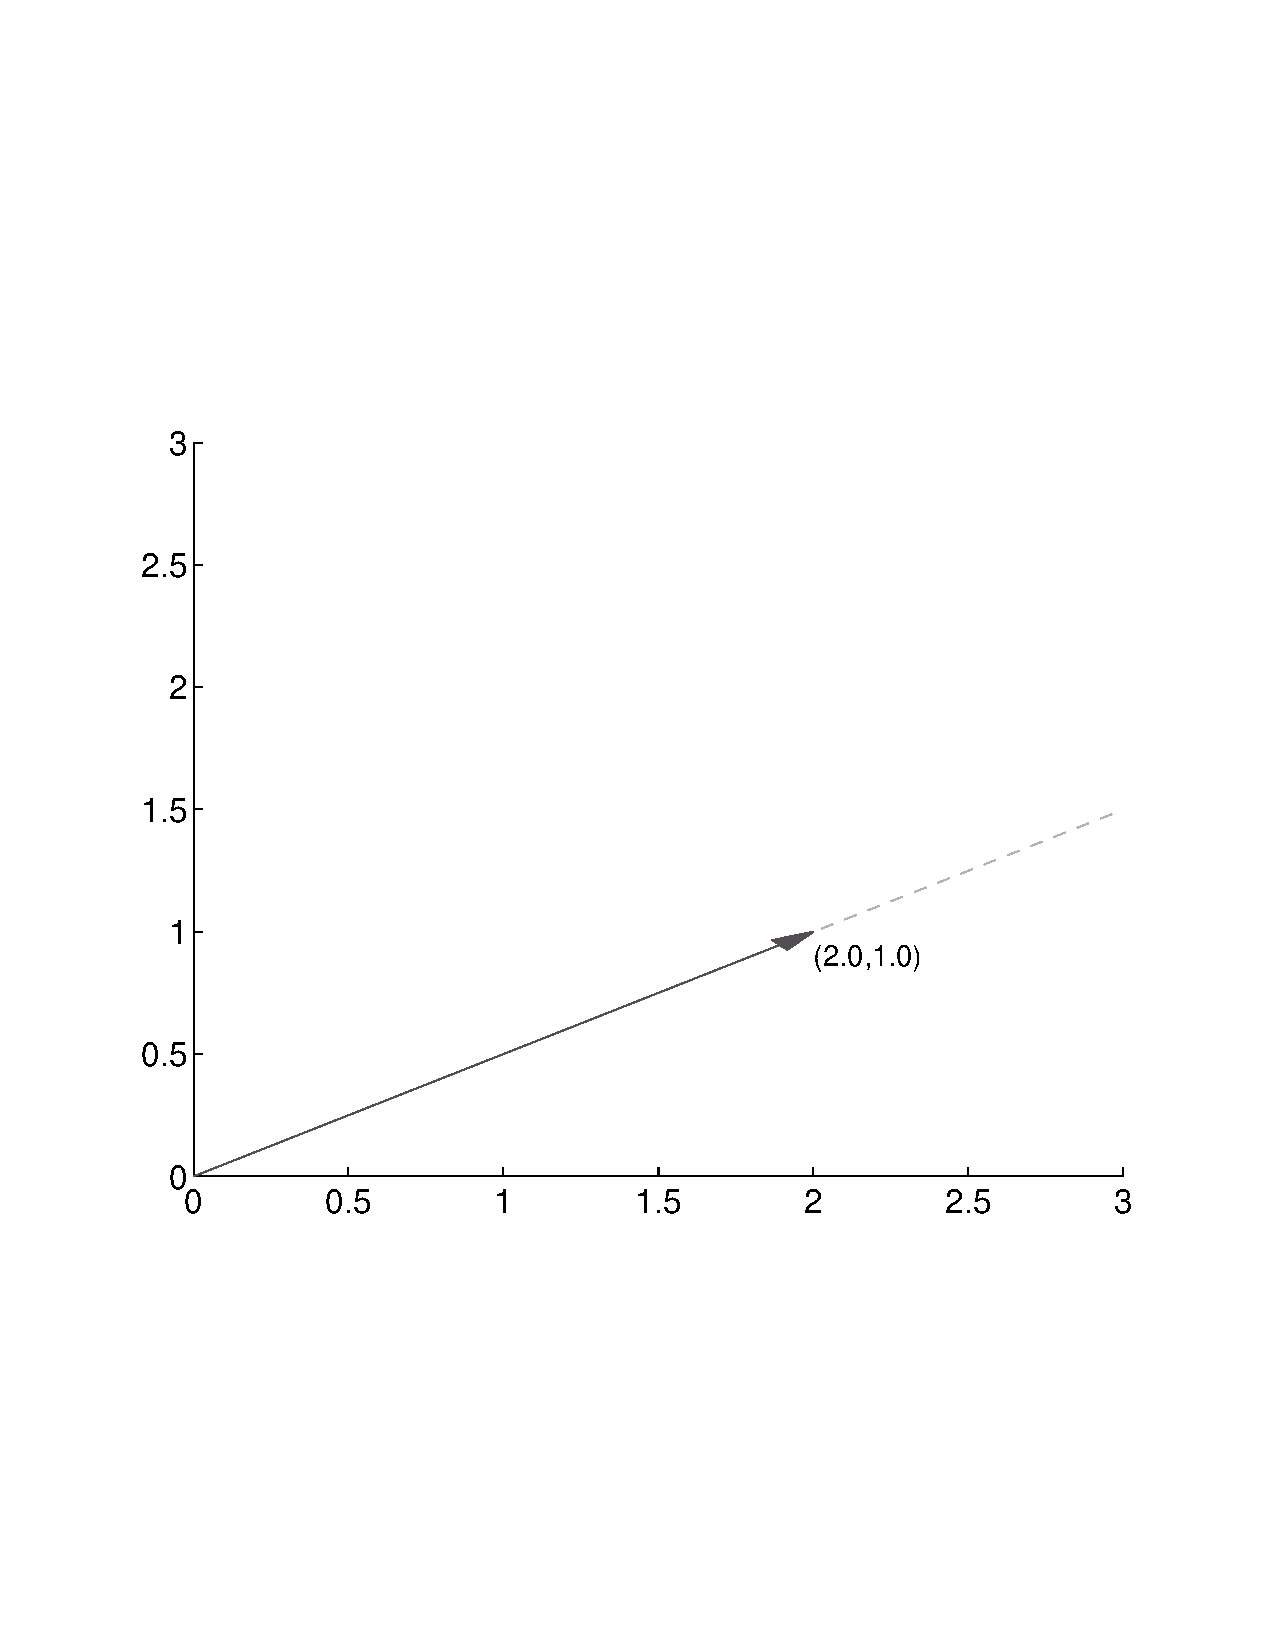
\includegraphics[scale=0.5, trim={2cm, 7cm, 2cm, 7cm}, clip]{Plots/StateSpaceGeometry1.pdf}
\end{figure}

Next suppose that there is some other vector $b=(1,1)$. We want to know
what is the \emph{projection} of blue line $b$ onto black line $a$.
How much does $b$ point in the $a$ direction? How much of movement in
direction $b$ can be ``explained'' by movement in direction $a$?
To answer these questions, project $b$ onto $a$.
\begin{figure}[htpb!]
  \centering
  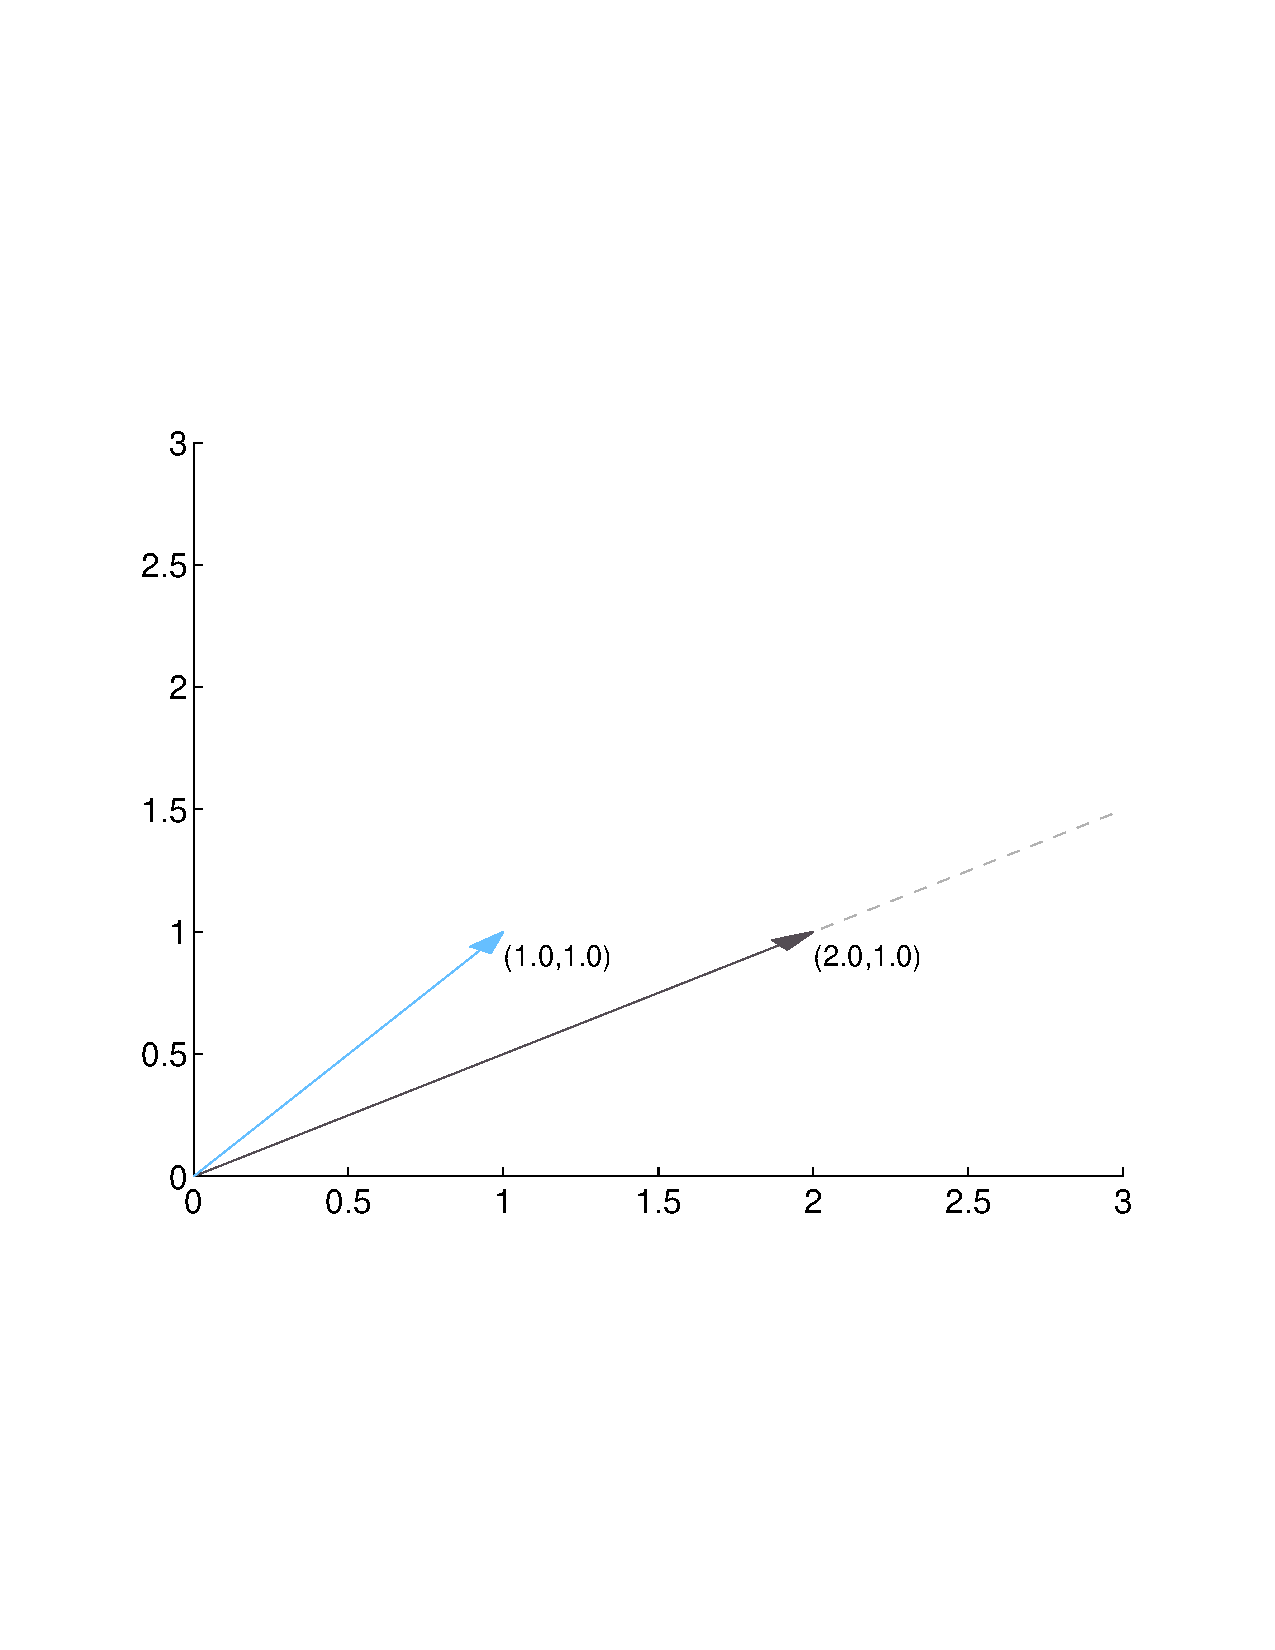
\includegraphics[scale=0.5, trim={2cm, 7cm, 2cm, 7cm}, clip]{Plots/StateSpaceGeometry2.pdf}
\end{figure}

Mathematically, projection just means ``linear regression without a
constant''
\begin{align*}
  b &= \beta a + \varepsilon \\\\
  \text{where}\qquad
  \beta &= (a'a)^{-1}a'b\\
  \varepsilon &= b - \beta \alpha
\end{align*}
So we can think of vector $b$ as the sum of some vector in the $a$
direction (i.e. $a$ rescaled by a constant $\beta$) plus some component
$\varepsilon$ completely unrelated to the direction of $a$.

Below, the blue vector (1.2,0.6) is the part of $b$ that points in the
$a$ direction ($\beta a$), while the orange vector is $\varepsilon$, the
part unrelated to the black line $a$ direction.

\begin{figure}[htpb!]
  \centering
  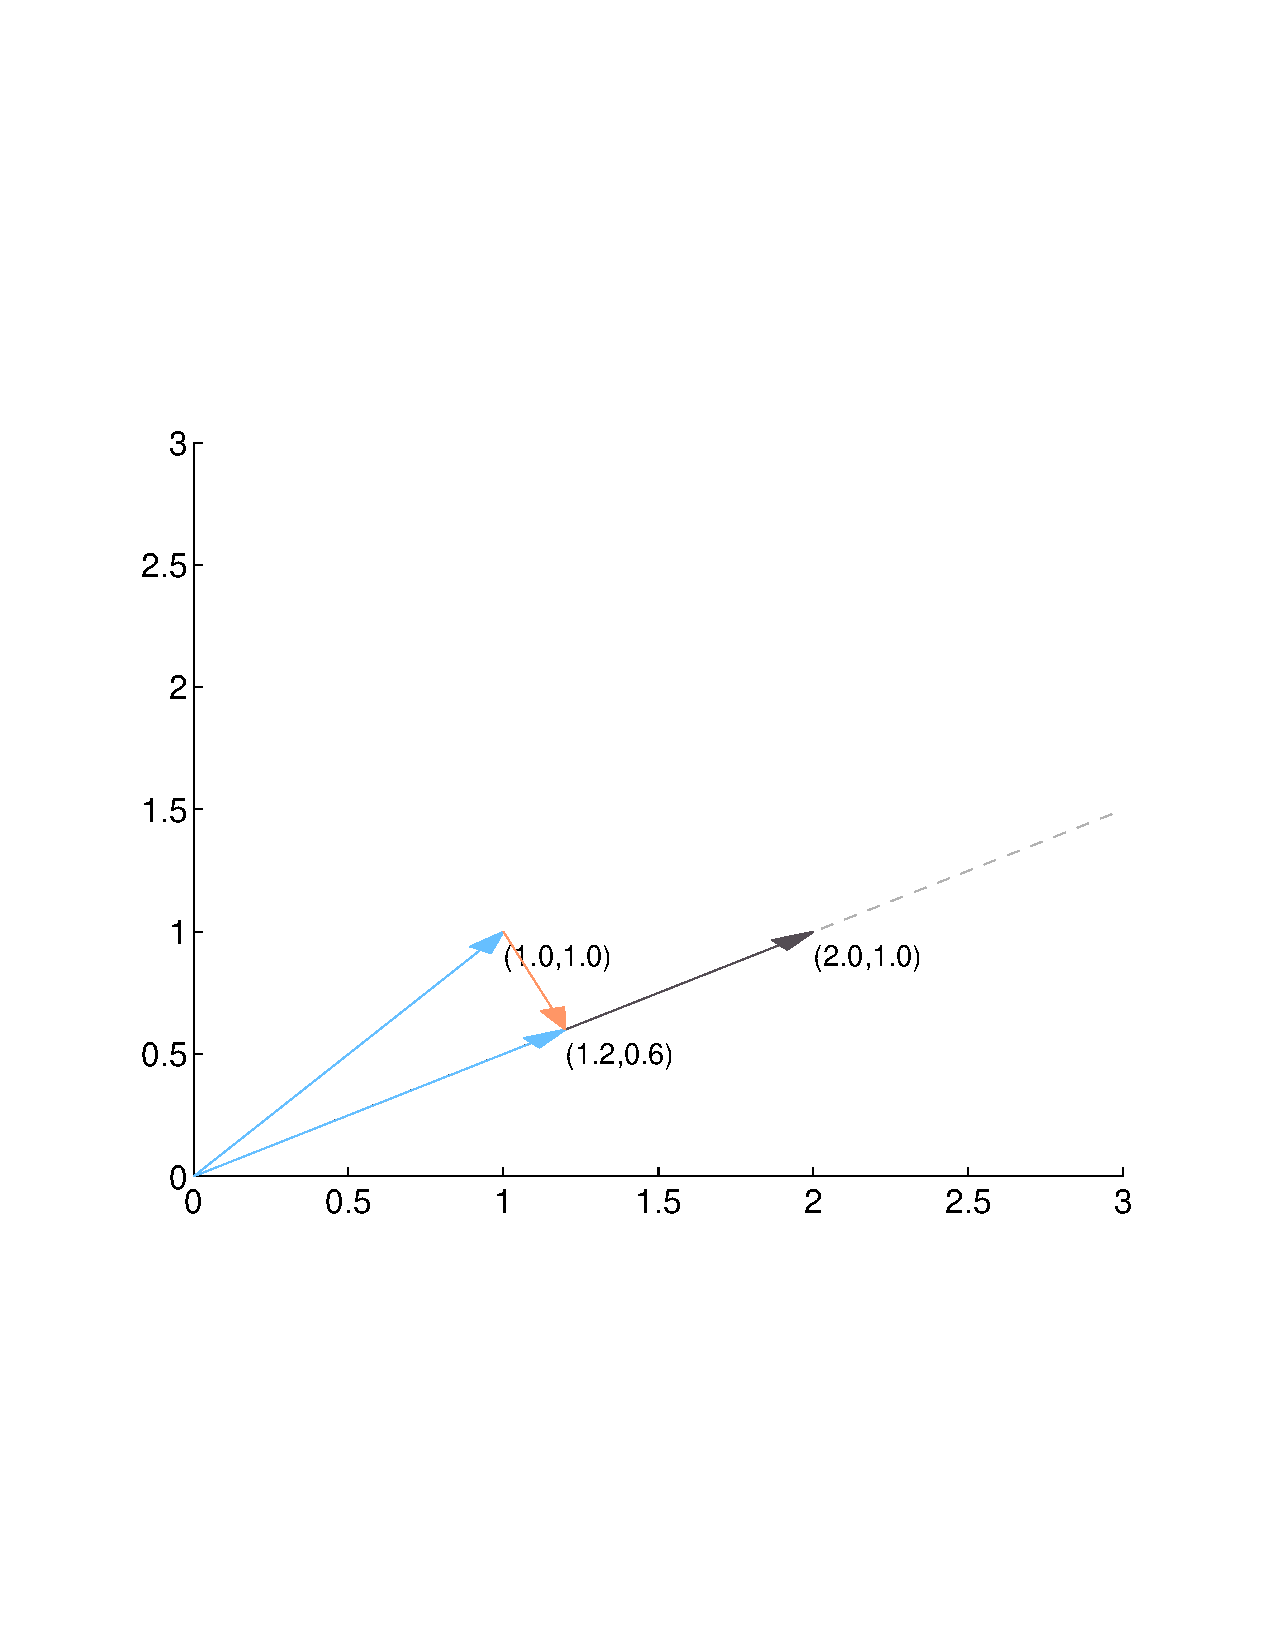
\includegraphics[scale=0.5, trim={2cm, 7.2cm, 2cm, 7.2cm}, clip]{Plots/StateSpaceGeometry3.pdf}
\end{figure}

Geometrically, projection also gives the closest point on black line $a$
to the tip of blue line $b$. As is typical, we find this point by
traveling on a straight line---the orange vector---from the tip of $b$
to some point on $a$, moving at \emph{right angles} to the direction of
$a$.  Motivated another way, the new dashed line below hits the tip of
$b$ while also intersecting $a$ at a right angle.
\begin{figure}[htpb!]
  \centering
  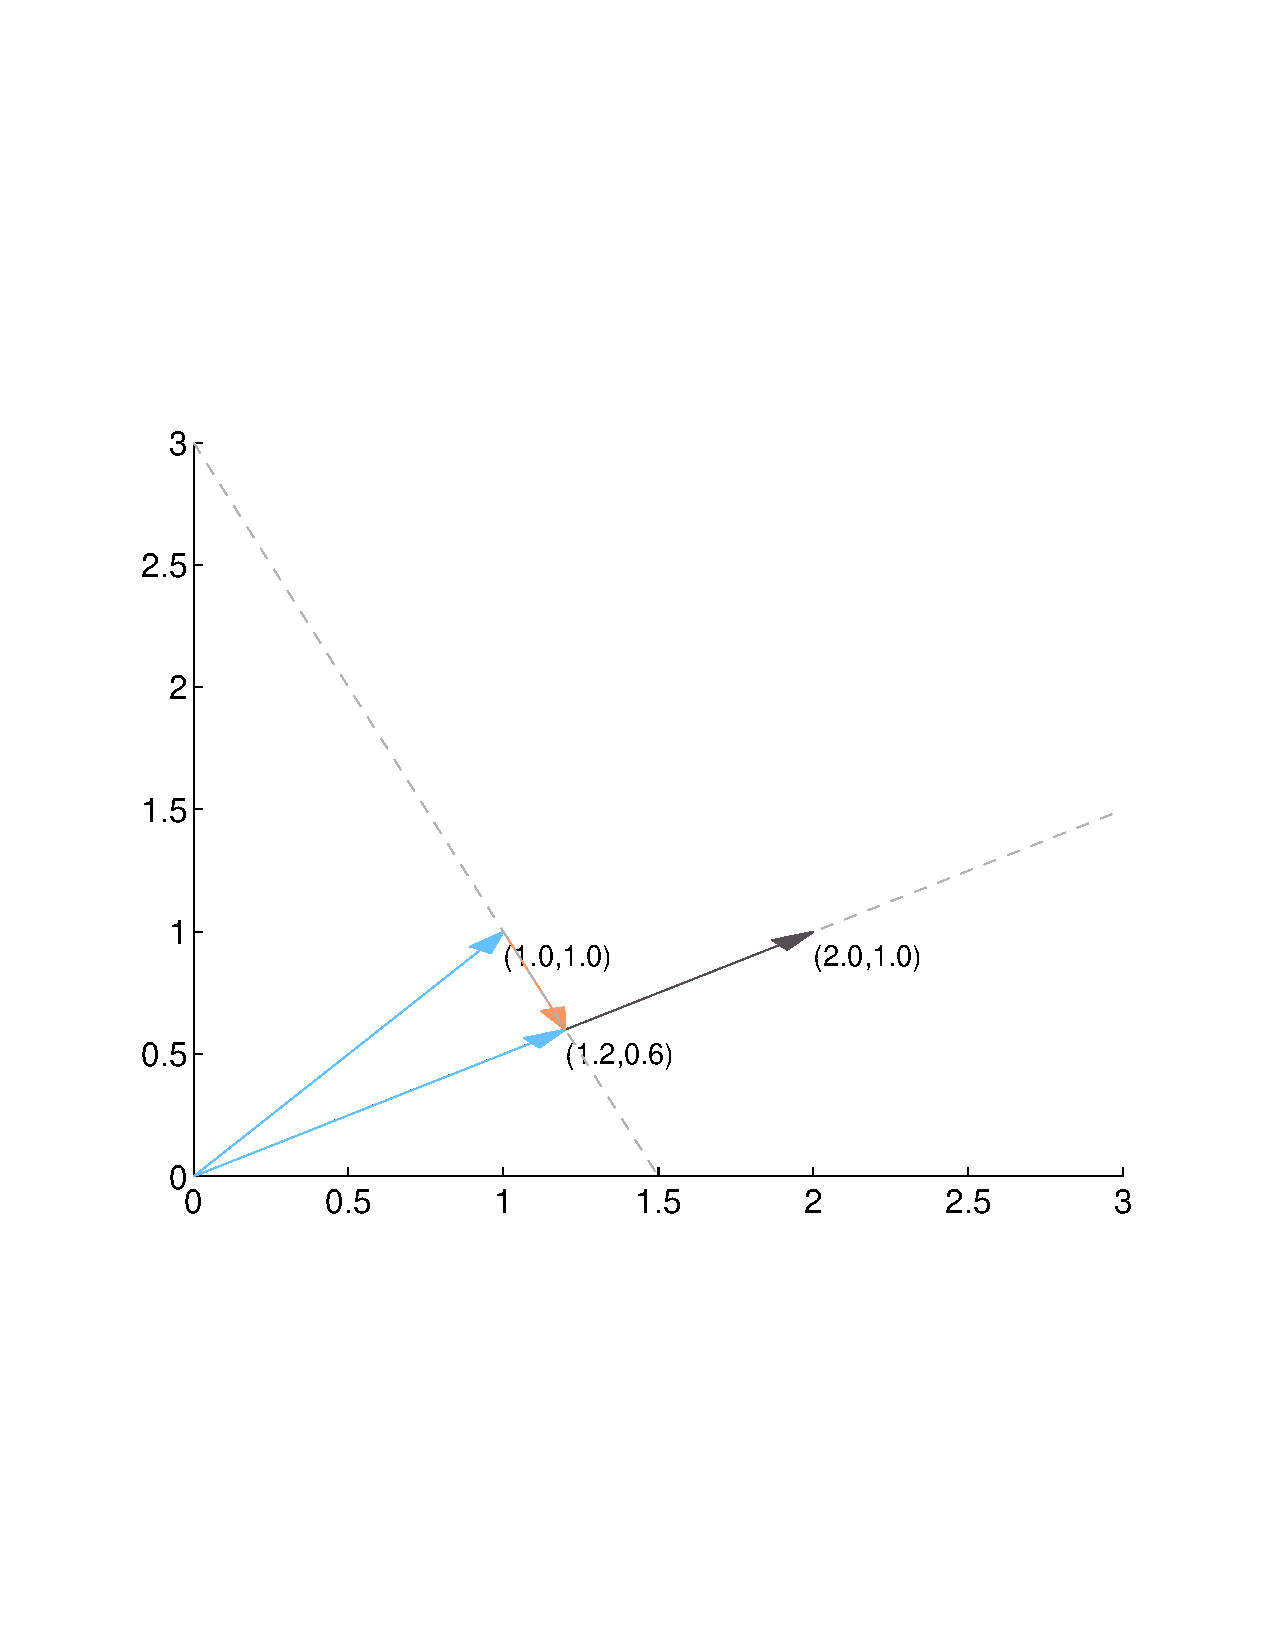
\includegraphics[scale=0.4, trim={2cm, 7.2cm, 2cm, 7.2cm}, clip]{Plots/StateSpaceGeometry4.pdf}
\end{figure}

\clearpage
Moreover, this dashed line extending infinitely in either direction from
the orange line traces out the set of all vectors that have an
\emph{identical} projection onto $a$. For every vector ending at some
point on this dashed line, the quickest right angle path to $a$ follows
the dashed line and lands at exactly the same point: (1.2,0.6).

\begin{figure}[htpb!]
  \centering
  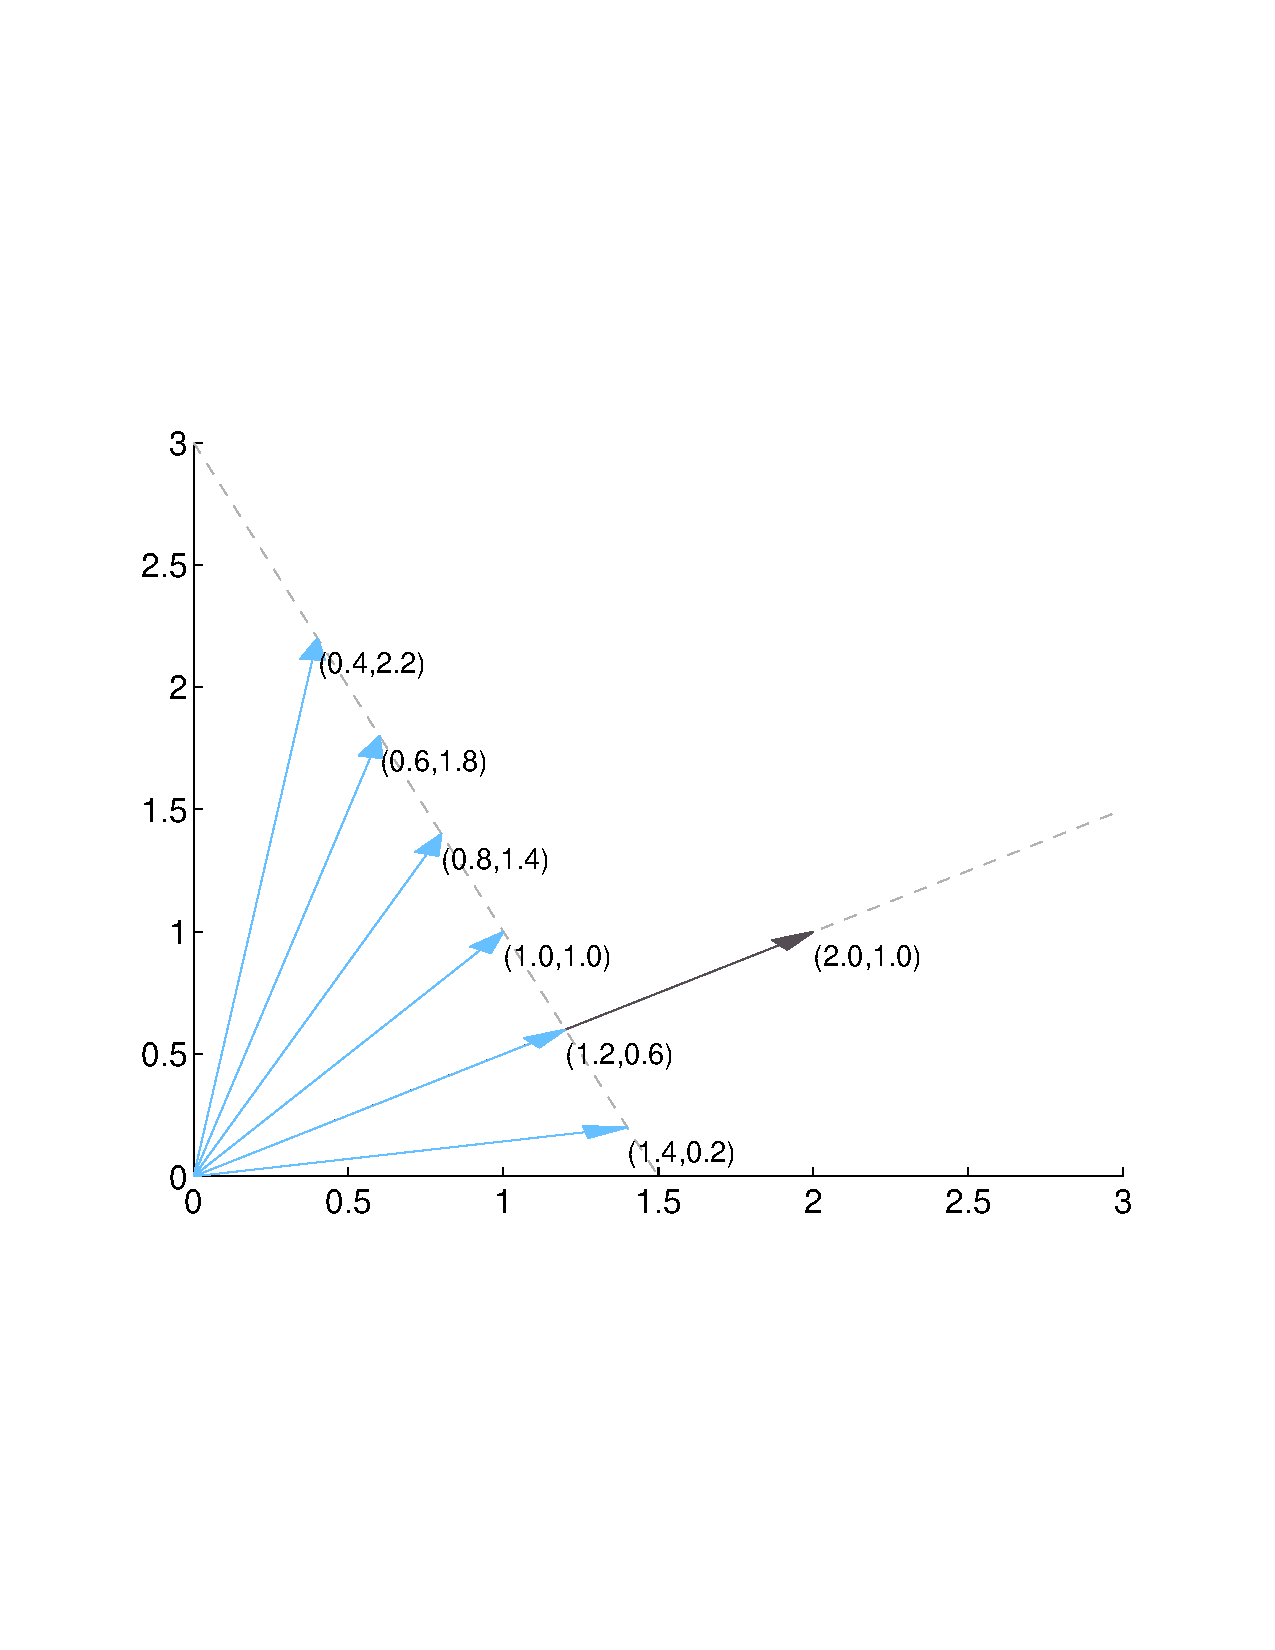
\includegraphics[scale=0.5, trim={2cm, 7cm, 2cm, 7cm}, clip]{Plots/StateSpaceGeometry5.pdf}
\end{figure}

But there are also infinitely many lines perpendicular to the direction
of $a$ (parallel to our original orange and dashed line). The figure
below shows one more example. This new dashed line traces out another
infinite set of vectors with an identical projection onto $a$.

\begin{figure}[htpb!]
  \centering
  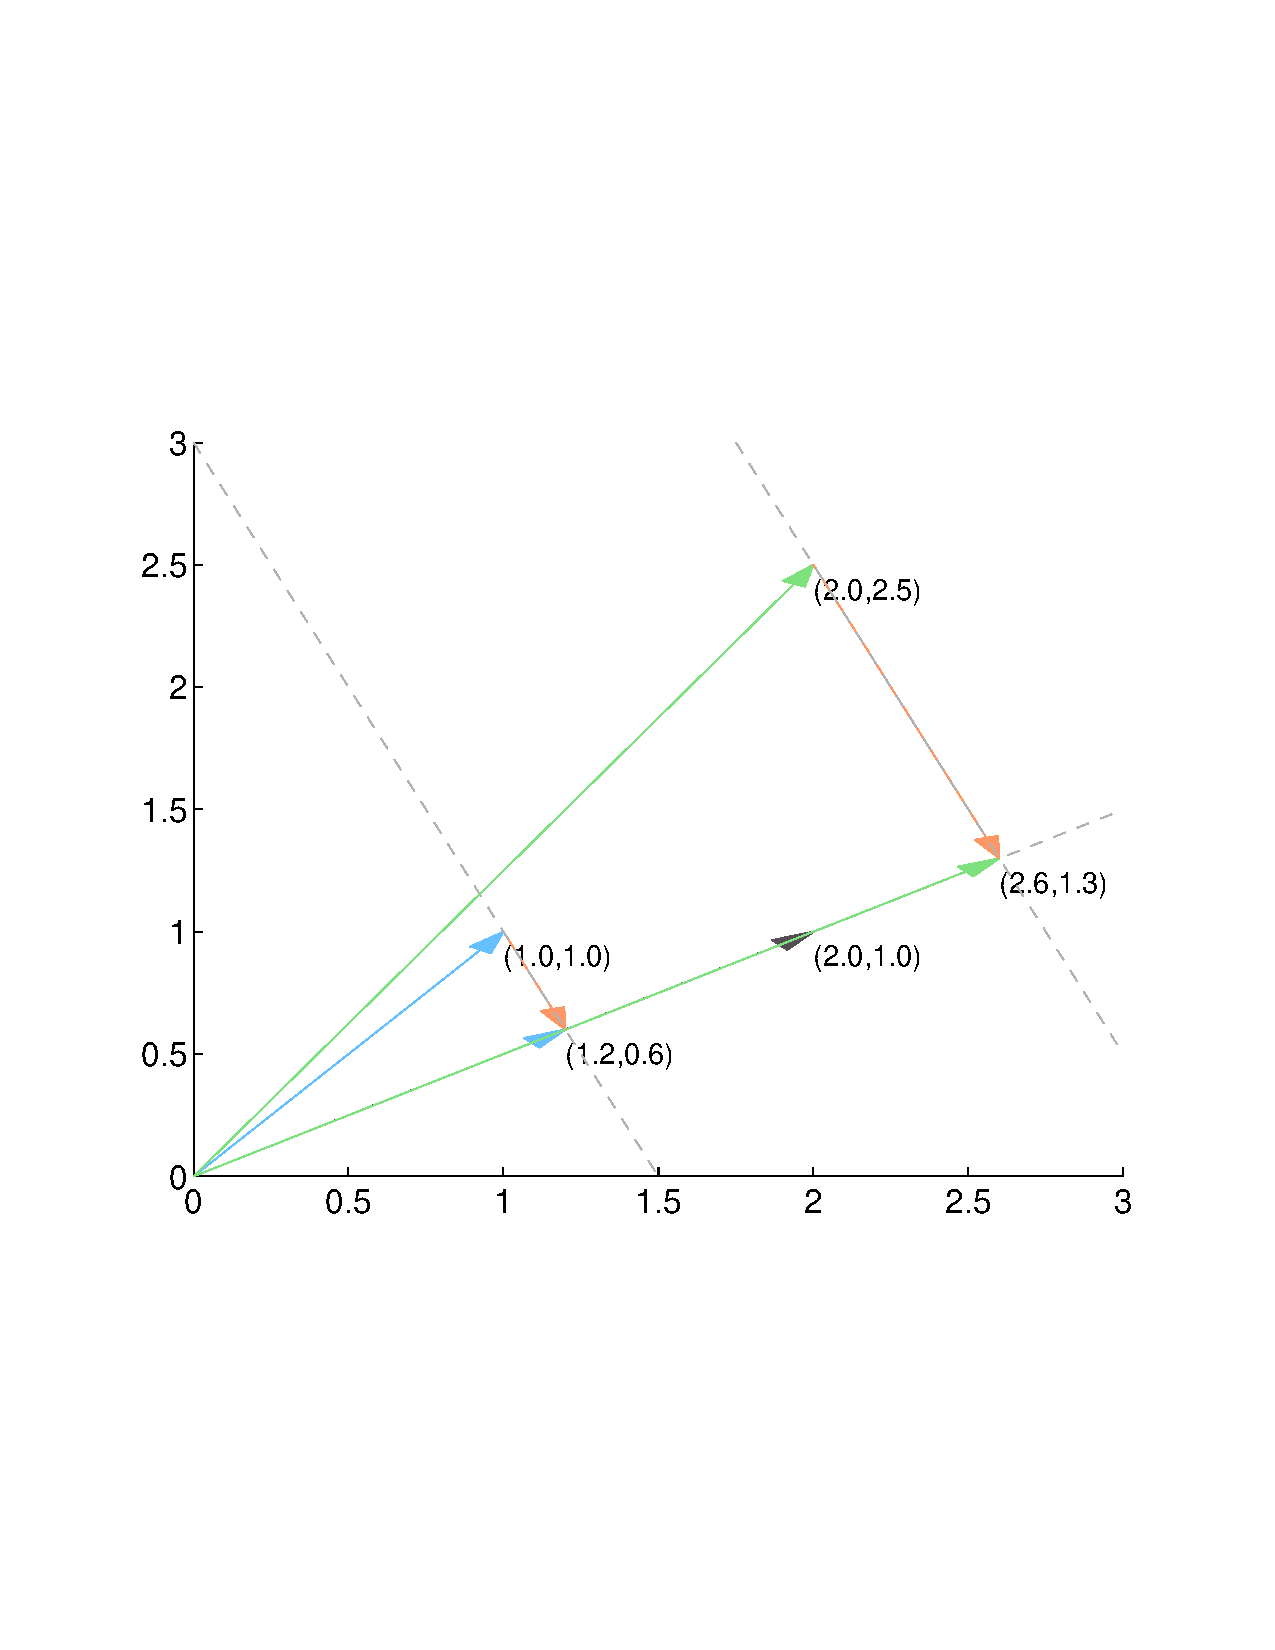
\includegraphics[scale=0.6, trim={2cm, 7cm, 2cm, 7cm}, clip]{Plots/StateSpaceGeometry6.pdf}
\end{figure}

Lastly, I just want to flip this logic around. Above, I defined
projection as ``Linear regression without a constant.'' Well, we can
think of linear regression in terms of projections. Write a regression
formula as
\begin{align*}
  y_i = \beta x_i + \varepsilon_i
\end{align*}
where $x_i$ is a vector of $k$ regressors that might include a constant
term. Think of $x_i$ as a point in $\mathbb{R}^k$, and think of
$\begin{pmatrix}y_i & x_i'\end{pmatrix}'$ as a point in
$\mathbb{R}^{k+1}$.

Now regression finds $\beta$ such that
\begin{enumerate}
  \item You minimize $\varepsilon_i$
  \item $\mathbb{E}[x_i\varepsilon_i]=0$
\end{enumerate}
You can do this by traveling in a straight line from the point
$\begin{pmatrix}y_i & x_i'\end{pmatrix}'$ in $\mathbb{R}^{k+1}$ to the
point $x_i$ in $\mathbb{R}^k$. That will be the ``quickest'' (i.e.\
smallest $\varepsilon_i$) route. Moreover, by traveling along this
straight line, you're traveling at a \emph{right angle} to point $x_i
\in \mathbb{R}^k$ so that $\mathbb{E}[x_i\varepsilon_i]=0$.

Geometrically, the projection of $y_i$ onto $x_i$ is really the
projection of point $\begin{pmatrix}y_i & x_i'\end{pmatrix}'$ onto
$x_i$, and it finds how much of the direction of $y_i$ can be
``explained'' by the direction of $x_i$. The $\varepsilon_i$ is simply
an extra residual that is completely unrelated to $x_i$ and its
direction.




\section{Price-Dividend and Return Linearizations}

We'll derive an approximation to an identity that says the following:
there are three potential reasons the price-dividend ratio might be
high:
\begin{enumerate}
    \item Investors expect dividends to rise.
    \item Investors expect low future returns, so future cashflows
	are discounted at a lower than usual rate. This leads
	to higher prices.
    \item Investors expect prices to rise forever, giving an
	adequate return even if there are no dividends.
\end{enumerate}
Now, we asserted above that Option 2 is the correct observation.
But how can we test that?  We'll, let's derive the identity that
lays out the theory behind Options 1-3.

\subsection{The Identity}

Start with the identity, and do some rearranging, letting $R$ equal
gross returns (price increases plus dividends), $D$ be dividends,
and $P$ be price.
\begin{align}
    1 &= R^{-1}_{t+1} R^{}_{t+1} = R^{-1}_{t+1} \frac{P_{t+1} + D_{t+1}}{P_t} \notag \\
    \Leftrightarrow \quad \frac{P_t}{D_t} &=
	R^{-1}_{t+1} \left( 1 + \frac{P_{t+1}}{D_{t+1}}\right) \frac{D_{t+1}}{D_t}
	\label{pdid} \\
    \Leftrightarrow \quad {P_t} &=
	R^{-1}_{t+1} \left( {D_{t+1}} + {P_{t+1}}\right)
	\label{pid}
\end{align}
Now, we can iterate forward Equation \ref{pid} and take a conditional
expectation to get
\begin{align}
    \label{pid2}
    P_t = E_t \sum^\infty_{j=1} \left(\prod^j_{k=1} R^{-1}_{t+k} \right)
	D_{t+j}
\end{align}
Now look at the previous line, and do the reverse of what we did
in going from Equation \ref{pdid} to Equation \ref{pid} (defining
$\Delta D_t := D_t / D_{t-1}$:
\begin{align}
    \Rightarrow \qquad \frac{P_t}{D_t} &= E_t \sum^\infty_{j=1}
	\left(\prod^j_{k=1} R^{-1}_{t+k} \right)  \frac{D_{t+j}}{D_t}
	\notag \\
    \Leftrightarrow \qquad \frac{P_t}{D_t} &= E_t \sum^\infty_{j=1}
	\left(\prod^j_{k=1} R^{-1}_{t+k} \right)
	\left(\prod^{j}_{k=1} \frac{D_{t+k}}{D_{t+k-1}}\right) \quad
	\text{Telescoping product trick!} \notag \\
    \Leftrightarrow \qquad \frac{P_t}{D_t} &= E_t \sum^\infty_{j=1}
	\left(\prod^j_{k=1} R^{-1}_{t+k} \Delta D_{t+k} \right)
	\label{pdid2}
\end{align}
So, what do we have? The identitiy in Equation \ref{pid2} tells us that
prices will increase if the discount rate \emph{falls} or if Expected
future dividends rise.  \emph{However}, prices aren't stationary, which
is why we went to the trouble of deriving the identity in
Equation \ref{pdid2}, which \emph{is} a stationary variable that
captures the same logic as \ref{pid2}, and can be estimated properly
via traditional time series approaches.


\subsection{The Linearization}

To make the identities derived above easier to handle, we take
logs to linearize!
Letting lowercase letters represent the logs of uppercase letters, we
get from Equation \ref{pdid}
\begin{align}
    \ln \frac{P_t}{D_t} &=
	\ln \left\{ R^{-1}_{t+1} \left( 1 + \frac{P_{t+1}}{D_{t+1}}\right) \frac{D_{t+1}}{D_t}
	\right\} \notag \\
	p_t - d_t &= -r_{t+1} + \ln( 1 + e^{p_{t+1} - d_{t+1}})
	+ \Delta d_{t+1} \label{approx}
\end{align}
Now do Taylor Expansion of the last term about a point $P/D = e^{p-d}$
(we'll use both the left- and righthand side of that point to
simplify, so watch out for that).  Also implicit in the
deriviation, I'll be evaluating the derivative in the second
term at $P/D = e^{d-d}$, so watch out for that too:
\begin{align*}
    f(p_t - d_t) &= \ln(1 + e^{p_{t+1} - d_{t+1}}) \\
    &\approx \ln(1 + e^{p - d}) +
	\frac{d\left[\ln(1 + e^{p_{t+1} - d_{t+1}})\right]}{d(p_t - d_t)}
	\cdot \left\{ (p_{t+1}-d_{t+1}) - (p-d) \right\} \\
    &= \ln(1 + e^{p - d}) +
	\frac{e^{p_{t+1} - d_{t+1}}}{1+e^{p_{t+1} - d_{t+1}}}
	\cdot \left\{ (p_{t+1}-d_{t+1}) - (p-d) \right\} \\
     &= \ln(1 + {P}/{D}) +
	\frac{P/D}{1+P/D}
	\cdot \left\{ (p_{t+1}-d_{t+1}) - (p-d) \right\} \\
    &= \ln(1 + {P}/{D}) +
	\rho\left\{ (p_{t+1}-d_{t+1}) - (p-d) \right\}
\end{align*}
So now let's just plug this log-linear approximation into Equation
\ref{approx}:
\begin{equation}
    p_t - d_t \approx -r_{t+1}
	+ \Delta d_{t+1} +  k +
	\rho\left\{ (p_{t+1}-d_{t+1}) - (p-d) \right\} \\
\end{equation}
where $k$ equals $\ln(1+P/D)$, which is a constant.\footnote{Note,
$\rho$ is just a constant of approximation that can be simplified
using the fact that dividend yields roughly 4\% on average, so
the Price/Dividend ratio is about 25:
    \[ \rho = \frac{P/D}{1+P/D} = \frac{1}{1+ D/P} \approx 1 - D/P = 0.96 \]
}
Now iterating forward is even more straightforward:
\begin{equation}
    \label{todec}
    p_t - d_t = C +  \sum^\infty_{j=1} \rho^{j-1} (\Delta d_{t+j}
	- r_{t+j})
\end{equation}
From this, it's clear that an ex-post high dividend-price ratio will result
only in the presence of high dividend growth or low subsequent returns.
To turn Equation \ref{todec} into an ex ante price-dividend ratio,
take expectations of everything on the right.


\newpage
\subsection{Decomposing the Variance}

To answer the question of what drives a high dividend-price ratio,
we'll decompose the variance in Equation \ref{todec} as follows:
\begin{align*}
    \text{Var}(p_t - d_t) = E\left[ (p_t - d_t) - E(p_t - d_t) \right]^2
    p_t - d_t = C +  \sum^\infty_{j=1} \rho^{j-1} (\Delta d_{t+j}
	- r_{t+j})
\end{align*}







%\cite{LabelInSourcesFile}
%\citep{LabelInSourcesFile} Cites in parens
%\nocite{LabelInSourceFile} includes in refs w/o specific citation
%\bibliographystyle{apalike}
%\bibliography{sources.bib} where sources.bib is file




\end{document}


%%%% INCLUDING FIGURES %%%%%%%%%%%%%%%%%%%%%%%%%%%%

   % H indicates here
   %\begin{figure}[h!]
   %   \centering
   %   \includegraphics[scale=1]{file.pdf}
   %\end{figure}

%   \begin{figure}[h!]
%      \centering
%      \mbox{
%	 \subfigure{
%	    \includegraphics[scale=1]{file1.pdf}
%	 }\quad
%	 \subfigure{
%	    \includegraphics[scale=1]{file2.pdf}
%	 }
%      }
%   \end{figure}


%%%%% Including Code %%%%%%%%%%%%%%%%%%%%%5
% \verbatiminput{file.ext}    % Includes verbatim text from the file
% \texttt{text}	  % includes text in courier, or code-like, font
